


To get started with reinforcement learning,
we need to define the most basic concept, the
\emph{environment} for the decision taking \emph{agent}.
This environment is formalized as a so called \emph{decision process}.
In order to define this we need the concept of a \emph{probability kernel}

\begin{defn}[Probability kernel]
  Let $\Cal{X}$ and $\cl{Y}$ be measurable spaces.
  A function
  \[ \kappa(\cdot \mid \cdot) : \Sigma_\Cal{Y} \times \Cal{X} \to [0,1] \]
  is an $\cl{X}$-\defemph{probability kernel}
  on $\cl{Y}$ provided
  \begin{enumerate}
    \item $B \mapsto \kappa(B \mid x) \in \Cal{P}(\cl{Y})$
      that is $\kappa(\cdot \mid x)$ is a probability measure
      for any $x \in \Cal{X}$.
    \item
      $x \mapsto \kappa(B \mid x) \in \Cal{M}(\Cal{X}, \Cal{Y})$
      that is $\kappa(B \mid \cdot)$ is $\Sigma_\Cal{X}$-$\Sigma_\Cal{Y}$
      measurable for any $B \in \Sigma_\Cal{Y}$.
  \end{enumerate}
  We write $\kappa : \Cal{X} \leadsto \Cal{Y}$.
  \label{defn:probKer}
\end{defn}
\begin{rem}
  Note that probability kernel $\kappa$ can also be viewed as a mapping
  $\kappa : \cl{X} \to \cl{P}(\cl{Y})$.
\end{rem}

Probability kernels are easily obtained by integration over suitable
measurable functions.

\begin{example}
  If $f : \cl{X} \times \cl{Y} \to [0,\infty)$
  is a positive measurable function with the property that
  \[ \forall x \in \cl{X} : \int f(x, y) \difd \mu(y) = 1 \]
  for some measure $\mu$ on $\cl{Y}$
  then $\kappa(B \mid x) = \int_B f(x, y) \difd \mu(y)$ defines a
  $\cl{X}$-probability kernel on $\cl{Y}$.
  This follows by basic measure theory and we omit these details.
\end{example}

A handy property of kernels is
\begin{prop}
  Let $\kappa : \Cal{X} \leadsto \Cal{Y}$ be a probability kernel
  and $f : \cl{X} \times \cl{Y} \to \R$ be measurable satisfying
  that $f(x, \cdot)$ is $\kappa(\cdot \mid x)$-integrable for every $x \in \cl{X}$.
  Then the map
  \[ x \mapsto \int f(x, \cdot) \difd \kappa(\cdot \mid x)\]
  is measurable into $(\R, \bb{B})$.
  \label{prop:intKerMeas}
\end{prop}
\begin{proof}
  This is a matter of going through the standard construction of the integral,
  noting that indicator functions $1_A$ on a measurable set $A \in \Sigma_\cl{X}$
  are measurable by \cref{defn:probKer}.2 since $\kappa$ is a kernel.
  Then extend by sums and limits.
\end{proof}

We can now state the definition of a decision process

\begin{defn}[History dependent decision process]
  A (countable)
  \defemph{history dependent decision process} (HDP) is determined by
  \begin{enumerate}
    \item $(\Cal{S}_n)_{n \in \N}$ a 
      measurable space of \defemph{states} for each timestep $n$.
    \item $(\Cal{A}_n)_{n \in \N}$ a 
      measurable space of \defemph{actions} for each timestep $n$.

      for each $n \in \N \cup \{\infty\}$
      define the \defemph{history} spaces
      \[ \Cal{H}_1 = \Cal{S}_1, \quad
      \Cal{H}_2 = \Cal{S}_1 \times \Cal{A}_1\times \Cal{S}_2 \]
      \[ \Cal{H}_n = \Cal{S}_1 \times \Cal{A}_1
	\times \Cal{S}_2 \times \Cal{A}_2
      \times \Cal{S}_3 \times \dots \times \Cal{S}_n \]
      \[
	\Cal{H}_\infty = \Cal{S}_1 \times \Cal{A}_1 \times \Cal{S}_2 \times
	\dots
      \]
    \item $(P_n)_{n \in \N}$ a sequence of
      $\Cal{H}_n \times \Cal{A}_n \leadsto \Cal{S}_{n+1}$ probability kernels
      called the \defemph{transition} kernels.
    \item $(R_n)_{n \in \N}$ a sequence of
      $\Cal{H}_{n+1} \leadsto \R$ probability kernels
      called the \defemph{reward} kernels.
    \item $\frak{A}_n(h_n) \subseteq \cl{A}_n$ a set of admissable actions
      for each $h_n \in \cl{H}_n$ and $n \in \N$.
  \end{enumerate}
  \label{sett:HDP}
\end{defn}

%todo example
With a HDP and an a way of choosing actions for each new state
we can obtain sequence of states, actions and rewards, that is
a history, by sampling from the kernels.
%todo example
To make precise what it means to choose actions we introduce the notion
of a \emph{policy}.

\begin{defn}[Policy]
  A (randomized) \defemph{policy} $\pi = (\pi_n)_{n \in \N}$ for a
  HDP is a sequence of probability kernels 
  $\pi_n : \Cal{H}_n \leadsto \Cal{A}_n$,
  such that $\pi_n(A(h_i) \mid h_i) = 1$ for alle $h_i \in \cl{H}_i$,
  i.e. the policy chooses only admissable actions (with probability 1).
  The set of all policies we denote $R\Pi$.
\end{defn}

With a HDP, and some distribution $\mu \in \cl{P}(\cl{S}_1)$
of the \emph{starting state} $S_1 \sim \mu$
and some policy $\pi$ intuitively we
should be able to obtain a history by sampling
\begin{itemize}
  \item an action $A_1 \in \frak{A}_1(S_1)$ from $\pi_1(\cdot \mid H_1)$
  \item a state $S_2 \in \cl{S}_2$ from $P(\cdot \mid S_1, A_1)$,
  \item an action $A_2 \in \frak{A}_2(S_1, A_1, S_2)$ from $\pi_2(\cdot \mid
    S_1, A_1, S_2)$
  \item and so on.
\end{itemize}

where $S_1, A_1, S_2, A_2, \dots$ 
And in fact we will now see that it is possible to use the transition
and reward kernels to obtain a measure on $\cl{H}_\infty$.
For this we need some additional measure theory on
probability kernels.

\begin{thm}[Integration of a kernel]
  Let $\mu \in \Cal{P}(\Cal{X})$ and $\kappa : \Cal{X} \leadsto \Cal{Y}$.
  Then there exists a uniquely determined probability measure
  $\lambda \in \Cal{P}(\Cal{X} \times \Cal{Y})$
  such that
  \[ \lambda(A \times B) = \int_A \kappa(B \mid x) \difd \mu(x) \]
  \label{thm:intKer}
  We denote this measure $\lambda = \kappa \mu$.
\end{thm}
\begin{proof}
  For $G \in \Sigma_\cl{X} \otimes \Sigma_\cl{Y}$ and $x \in \cl{X}$ define
  $G^x \defeq \{ y \in \cl{Y} \mid (x, y) \in G \} $.
  It is easy to check that the map $x \mapsto \kappa(G^x \mid x)$ is
  measurable, using a Dynkin class argument.
  Thus we can define
  \[ \lambda(G) = \int \kappa(G^x \mid x) \difd \mu(x) \]
  Immedially we see that
  $\lambda(\cl{X} \times \cl{Y}) = 1$.
  Let $G_1, G_2, \dots \in \Sigma_\cl{X} \otimes \Sigma_\cl{Y}$ be
  mutually disjoint.
  Then $G_1^x, G_2^x, \dots$ are mutually disjoint aswell.
  So by monotone convergence
  \[ \lambda \left( \bigcup_{i \in \N} G_i \right)
  = \int \kappa\left( \bigcup_{i=1}^\infty G_i^x \Mid x \right) \difd \mu(x)
    = \int \sum_{i=1}^\infty \kappa(G^x_i \mid x) \difd \mu(x)
  = \sum_{i=1}^\infty \lambda (G_i) \]
  Uniqueness follows because the property
  \[ \lambda(A \times B) = \int_A \kappa(B, x) \difd \mu(x) \]
  should hold on the all product sets, which form an
  intersection-stable generating collection for
  $\Sigma_\cl{X} \otimes \Sigma_\cl{Y}$.
\end{proof}

\begin{rem}
  In light of \cref{thm:intKer} we can view a probability kernel as a mapping
  $\kappa : \cl{P}(X) \to \cl{P}(\cl{X} \times \cl{Y})$
  defined by $\mu \mapsto \kappa \mu$.
  \label{rem:measureMap}
\end{rem}

For an idea how to actually compute integrals over kernel derived measures
we here include
\begin{thm}[Extended Tonelli and Fubini]
  Let $\mu \in \Cal{P}(\Cal{X})$,
  $f \in \Cal{M}(\Sigma_\Cal{X} \otimes \Sigma_\Cal{Y}, \bb{B})$
  be a measurable function and
  $\kappa : \Cal{X} \leadsto \Cal{Y}$ be a probability kernel.
  Then
  \[ \int \abs{f} \difd \kappa \mu
  = \int \int \abs{f} \difd \kappa(\cdot \mid x) \difd \mu(x) \]
  Furthermore if this is finite, i.e. $f \in \Cal{L}_1(\kappa(\cdot, \mu))$
  then $A_0 \defeq \left\{ x \in \Cal{X} \Mid
    \int f \difd \kappa(\cdot \mid x) < \infty \right\}
  \in \Sigma_\Cal{X}$
  with $\mu(A_0) = 1$, 
  \[ x \mapsto \begin{cases}
      \int f \difd \kappa(\cdot \mid x) & x \in A_0
      \\ 0 & x \not\in A_0
  \end{cases} \]
  is $\Sigma_\Cal{X}$-$\bb{B}$ measurable and
  \[ \int f \difd \kappa \mu
  = \int_{A_0} \int f \difd \kappa(\cdot \mid x) \difd \mu(x) \]  
  \label{thm:extTonFub}
\end{thm}
\begin{proof}
  We refer to \ncite{RH14} thm. 1.3.2 and 1.3.3.
\end{proof}

\begin{prop}[Composition of kernels]
  Let $\kappa : \cl{X} \leadsto \cl{Y}$ and
  $\phi : \cl{X} \times \cl{Y} \leadsto \cl{Z}$ be probability kernels.
  Then there exists a unique probability kernel
  $\phi \kappa: \cl{X} \leadsto \cl{Y} \times \cl{Z}$
  satisfying
  \[ \phi \kappa(B \times C \mid x) = \int 1_B(y) \phi(C \mid x, y)
  \difd \kappa(y \mid x), \quad B \in \Sigma_\cl{Y}, \; C \in \Sigma_\cl{Z} \]
  called the \defemph{composition} of $\phi$ and $\kappa$.
  The composition is associative,
  that is if $\psi : \cl{X} \times \cl{Y} \times \cl{Z}
  \leadsto \cl{W}$
  is another probability kernel, then
  $(\psi \phi) \kappa = \psi (\phi \kappa)$.
  Associativity extends to measures, that is if
  $\mu \in \cl{P}(\cl{X})$ is a probability measure then
  $\phi (\kappa \mu) = (\phi \kappa) \mu$.
  Furthermore if $f : \cl{X} \times \cl{Y} \times \cl{Z} \to \R$ is
  a measurable function such that $f(x, \cdot, \cdot)$ is
  $\phi \kappa( \cdot \mid x )$-integrable then
  \[ \int f(x, y, z) \difd \phi \kappa (y, z \mid x)
  = \int \int f(x, y, z) \difd \phi(z \mid x, y) \difd \kappa(y \mid x) \]
  \label{prop:compKer}
\end{prop}
\begin{proof}
  See \cref{proof:compKer}.
\end{proof}

\begin{rem}
  A kernel $\varphi:\cl{Y} \leadsto \cl{Z}$
  can also be considered a kernel
  $\varphi' : \cl{X} \times \cl{Y} \leadsto \cl{Z}$
  by defining
  $\varphi'(\cdot \mid x, y) = \kappa(\cdot \mid y)$
  that is ignoring the first input.
  Therefore we can use \cref{prop:compKer} on $\varphi'$ to get
  $\varphi \kappa : \cl{X} \leadsto \cl{Y} \times \cl{Z}$.
  Projection $\rho_\cl{Z}$ onto $\cl{Z}$ also preserves the kernel property,
  so $\rho_\cl{Z}(\varphi' \kappa) : \cl{X} \leadsto \cl{Z}$ is
  yet another probability kernel.
  We denote this $\varphi \circ \kappa = \rho_\cl{Z}(\varphi' \kappa)$
  and this is also called \emph{composition of kernels} by some authors.
  In fact $\circ$ makes the class of measurable spaces
  into a category \mcite{L62},
  with identity $\id_{\Cal{X}}(\cdot \mid x) = \delta_x$.
\end{rem}

\subsubsection{From kernels to processes}

Throughout this section let $(\Cal{X}_n)_{n \in \N}$ be a sequence
of measurable spaces. For each $n \in \N$ let
$\kappa_n : \Cal{X}^{\ul{n}} \leadsto \Cal{X}_{n+1}$ be a probability kernel.

\begin{prop} For all $n \in \N$ the composition
  $\kappa_n \dots \kappa_1$ yields a $\cl{X}_1$-probability
  kernel on $\cl{X}_2 \times \dots \times \cl{X}_{n+1}$.
  \label{prop:kappaN}
\end{prop}
\begin{proof}
  This is by induction using \cref{prop:compKer}.
\end{proof}

\Cref{prop:kappaN} allows us to make sense to finite decision processes.
That is for any
$n \in \N$, distribution $\mu \in \cl{P}(\cl{S}_1)$ of $S_1$ 
and policy $(\pi_1, \pi_2, \dots) \in R\Pi$ we can get a distribution
of the $n$th history $H_n \in \cl{H}_n$ by the composition of kernels
\[ P_{n-1} \pi_{n-1} 
\dots P_2 \pi_2 P_1 \pi_1 \mu \in \cl{P}(\cl{H}_n) \]
We would like to extend this to a distribution on $\cl{H}_\infty$.
To do this we will need

\begin{thm}[Ionescu-Tulcea extension theorem]
  For every $\mu \in \Cal{P}(\Cal{X}_1)$ 
  there exists a unique probability measure
  $\rho \in \Cal{P}(\Cal{X}^{\ul{\infty}})$ such that
  \[ \kappa^{\ul{n-1}} \mu (A_1 \times A_2 \times \dots \times A_n) = \rho
    \left( A_1 \times A_2 \times \dots \times A_n \times
    \prod_{k=n+1}^\infty \Cal{X}_k \right)
  , \qquad \forall A \in \Sigma_{\Cal{X}^{\ul{n}}}, n \in \N \]
  \label{thm:ionescuTulcea}
\end{thm}
\begin{proof}
  We refer to \mcite{K02} thm. 5.17. %todo do the proof instead
\end{proof}

In particular \cref{thm:ionescuTulcea} applied to the measure Dirac-measure
$\delta_x$ can be interpreted as starting the process in $x \in \cl{X}_1$.
Later we would like to consider function defined

\begin{prop}[Ionescu-Tulcea kernel]
  Let $\mu_x$ denote the Ionescu-Tulcea measure of a
  sequence of probability kernels
  $\kappa_i : \Cal{X}^{\ul{i}} \to \Cal{X}_{i+1}$
  with starting measure $\delta_x$ on $\Cal{X}_1$ for any $x \in \Cal{X}_1$.
  Then $\kappa(A \mid x) = \mu_x(\cl{X}_1 \times A)$ defines a probability kernel
  $\kappa : \Cal{X}_1 \leadsto \Cal{X}_2 \times \cl{X}_3 \times \dots$.
\end{prop}
\begin{proof}
  Since we already know by \cref{thm:ionescuTulcea}
  that $\mu_x$ is a probability measure for any
  $x \in \Cal{X}_1$,
  we just have to show that $\kappa(A \mid x) = \mu_x(A)$ is measurable
  as a function of $x$ for all
  $A \in \Sigma$ where $\Sigma = \bigotimes_{i=2}^\infty \Sigma_{\Cal{X}_i}$.
  Let $\phi_A = x \mapsto \mu_x(A)$
  for all $A \in \Sigma$ and define
  \[ \bb{G} = \left\{ A \in \Sigma
  \Mid \phi_A \in \Cal{M}(\Cal{X}_1, [0,1]) \right\} \]
  The cylinder sets
  \[ \bb{O} = \left\{ A_2 \times \dots \times A_i \times \Cal{X}_{i+1},
  \dots \Mid A_i \in \Sigma_{\Cal{X}_i}, i-1 \in \N \right\} \]
  is a generator for $\Sigma$ stable under 
  finite intersections.
  By contruction $\bb{O} \subseteq \bb{G}$ since
  \[ \phi_{A_2 \times \dots \times A_i \times \Cal{X}_{i+1} \times \dots}
  = \kappa^{\ul{i-1}}(A_2 \times \dots \times A_i \mid \cdot) \]
  and any $\kappa^{\ul{i-1}}$ is a kernel making that function measurable.
  We will show that $\bb{G}$ is a Dynkin class.
  Then by Dynkins $\pi$-$\lambda$ theorem (see \cref{thm:DynkinPiLambda})
  \[ \sigma(\bb{O}) = \Sigma
  \subseteq \bb{G} \]
  implying that $\phi_A$ is measurable
  for all $A \in \Sigma$.
  
  For showing that $\bb{G}$ is a Dynkin class, notice that
  clearly $\Cal{X}_2 \times \cl{X}_3 \times \dots$ and $\emptyset$
  are in $\bb{G}$.
  If $A,\; B \in \bb{G}$ with $A \subseteq B$ then
  $\phi_{B \setminus A} = \phi_B - \phi_A \in \bb{G}$.
  Finally if $(B_n)_{n \in \N}$ is an ($\subseteq$-) increasing sequence
  in $\bb{G}$ then $\phi_{\bigcup_{n=1}^\infty B_n} =
  \lim_{n \to \infty} \phi_{B_n}$ is again measurable as it is a
  limit of measurable functions, showing that $\bb{G}$ is a Dynkin class.
\end{proof}

We will denote the Ionescu-Tulcea kernel $\dots \kappa_2 \kappa_1$ or
$\prod_{i=1}^\infty \kappa_i$ or simply $\kappa^{\ul{\infty}}$.
The next lemma will come in handy when manipulating with integrals over
kernel derived measures.

\begin{lem}
  The Ionescu-Tulcea kernel satisfies
  $\prod_{i=1}^\infty \kappa_i = (\prod_{i=2}^\infty \kappa_i) \kappa_1$.
  \label{lem:ionescu}
\end{lem}
\begin{proof}
  Let $x \in \Cal{X}_1$.
  Since for the composition of finitely many
  kernels by associativity (\cref{prop:compKer}) it holds that
  $\kappa_n \dots \kappa_1
  = (\kappa_n \dots \kappa_2) \kappa_1$.
  Therefore for any $n \in \N$ and $A \in \Sigma_{\cl{X}_2} \otimes
  \dots \otimes \Sigma_{\cl{X}_n}$, using \cref{thm:ionescuTulcea} we have
  \begin{align*}
    \left( \prod_{i=1}^\infty \kappa_i \right)
    \left( A \times \prod_{k=n+1}^\infty \Cal{X}_k \Mid x \right)
    = (\kappa_{n-1} \dots \kappa_2) \kappa_1 (A \mid x)
    &= \left( \left( \prod_{i=2}^\infty \kappa_i \right) \kappa_1 \right)
    \left( A \times \prod_{k=n+1}^\infty \Cal{X}_k \Mid x \right)
  \end{align*}
  for all $n \in \N$ and $A \in \Sigma_{\Cal{X}^{\ul{n}}}$.
  By the uniqueness in \cref{thm:ionescuTulcea} we are done.
\end{proof}

Let $\mu \in \cl{P}(\cl{S}_1)$ be a measure on the first state space.
By \cref{thm:ionescuTulcea} a HDP and a policy
$\pi = (\pi_1, \pi_2, \dots) \in R\Pi$ gives rise to
a kernel $\kappa_\pi : \cl{P}(\cl{S}_1) \to \cl{P}(\cl{H}_\infty)$, namely
\begin{equation}
  \kappa_\pi = \dots P_2 \pi_2 P_1 \pi_1 \mu
  \label{eq:kappaPi}
\end{equation}
In particular $\kappa_\pi \mu$ can be interpreted as the stochastic process
arising from sampling the first state from $\mu$ and then follow $\pi$
for a countable number of steps.
We will denote expectation with respect to $\kappa_\pi \mu$ by
$\E_{\mu}^\pi$. 
In the case where $\mu = \delta_{s}$ for some $s \in \cl{S}_1$
integration with respect to the measure $\kappa_\pi \delta_s$
and $\kappa_\pi(\cdot \mid s)$ is equivalent in the sense that
\[ \int f(s, a_1, s_2, \dots) \difd \kappa_\pi(a_1, s_2, \dots \mid s)
= \int f(s_1, a_1, s_2, \dots) \difd \kappa_\pi \delta_s(s_1, a_1, \dots) \]
Both of these measures can be interpreted as the stochastic process
arising from starting in state $s$ and following policy $\pi$.
We will sometimes abuse notation slightly, writing
$\kappa_\pi \delta_s = \kappa_\pi s$ and $\E_{\delta_s}^\pi = \E_s^\pi$.

\section{Policy evaluation and value functions}
The next step is to evaluate how \emph{good} a policy is.
This is where the reward kernels $R_1, R_2, \dots$ come into play.
However their stochastic properties will not be
relevant for this section. For now we will
only care about their expected values. Therefore we will need
\begin{asm}[Finite reward bound]
  For each $n \in \N$ there exists a bound $R_{\max, n} > 0$
  such that for all $h_n \in \cl{H}_n$ it holds that
  \[ R_n([-R_{\max, n}, R_{\max, n}] \mid h_n) = 1 \]
  \label{asm:finRewBound}
\end{asm}
This is assumed in the rest of this section and all following sections.
\begin{rem}
  \Cref{asm:finRewBound} implies that all $R_n(\cdot \mid h_n)$ has moments of
  all orders for any $h_n \in \cl{H}_n$.
  \label{rem:expRewMeas}
\end{rem}
\begin{defn}
  We define for each $n \in \N$
  \[ r_n : \cl{H}_n \to \R, \quad r(h_n) = \int x \difd R_n(x \mid h_n) \]
  called the $n$th \defemph{expected reward function}.
  \label{defn:expRewFunc}
\end{defn}
\begin{rem}
  The expected reward function $r_n$ is measurable due to
  \cref{prop:intKerMeas}.
\end{rem}

We are now ready to talk about \emph{value functions}.
A value function is any function $V: \cl{S}_1 \to \R$
which assigns a real number to a starting state (a state in $\cl{S}_1$).
An important class of value functions are the
policy evaluations:

\begin{defn}[Finite policy evaluation]
  We define the function $V_{n, \pi} : \cl{S}_1 \to \R$ by
  \[ V_{n,\pi}(s_1) = \E_{s_1}^\pi \sum_{i=1}^n r_i
    = \int \sum_{i=1}^n r_i(s_1, a_1, \dots, a_{i-1}, s_i)
  \difd \kappa_\pi s_1 \]
  called the $k$th \defemph{finite policy evaluation}.
  When $n=0$ we say $V_{0,\pi} = V_0 \defeq 0$ for any $\pi$.
\end{defn}
The finite policy evaluation
measures the expected total reward of starting in state $s_1 \in \cl{S}_1$
and then following the policy $\pi$ for $n$ steps.

We would like to extend this to an infinite policy evaluation
i.e. letting $n$ tend to $\infty$. To ensure that the integral is well-defined
we introduce the following conditions
\begin{asm}[Discounting] There exist a bound $R_{\max} > 0$ and a
  $\gamma \in [0,1)$ called the \defemph{discount} factor such that
  $R_i([-R_{\max} \gamma^i, R_{\max} \gamma^i] \mid h_{i+1}) = 1$,
  $\forall h_{i+1} \in \Cal{H}_{i+1},\; i \in \N$.
  \label{asm:D}
\end{asm}
This assumption allows the following definition of the following value function
\begin{defn}
  We define the (infinite) \defemph{policy evaluation} by
  \begin{equation}
    V_\pi(s) = \E_s^\pi \lim_{n \to \infty} \sum_{i=1}^n r_i
    = \int \sum_{i=1}^\infty r_i \difd \kappa_\pi s
    \label{eq:defInfPolEval}
  \end{equation}
\end{defn}
\begin{rem}
  In \cref{eq:defInfPolEval}
  it is implicit that for each $i \in \N$ the reward
  $r_i$ in the sum is applied 
  the $h_{i+1}$th history as a integration variable
  from the measure $\kappa_\pi s$.
\end{rem}
The infinite policy evaluation $V_\pi$ measures the expected total
reward after following the policy $\pi$ an infinite number of steps.
Whenever we work with the infinite policy evaluation we will
always make \cref{asm:D}.
We now mention some immediate properties of the finite and infinite
policy evaluations
\begin{prop} Let \cref{asm:D} hold. Then
  \leavevmode
  \begin{enumerate}
    \item $V_{n,\pi}, V_\pi$ are integrable with respect to
      $\kappa_\pi(\cdot \mid s)$
      for any $\pi \in R\Pi$ and any $s \in \cl{S}_1$.
    \item $\lim_{n\to\infty} V_{n, \pi} = V_\pi$
      for all $\pi \in R\Pi$.
    \item For any $\pi \in R\Pi$
      \[\abs{V_{n,\pi}}, \abs{V_\pi} \leq R_{\max} (1 - \gamma) < \infty\]
      \label{item:firstV3}
  \end{enumerate}
  \label{prop:VpiMeas}
\end{prop}
\begin{proof}  
  \leavevmode
  \begin{enumerate}
    \item By \cref{rem:expRewMeas} the expected reward functions
      are measurable. Therefore sums and limits of them are aswell
      se \cref{prop:intKerMeas}.
      Integrability follows once we show \cref{item:firstV3}.
    \item By monotone or dominated convergence.
    \item For any $\pi \in R\Pi$
      \[ \abs{V_\pi(s)} \leq \E_s^\pi \sum_{i \in \N} \abs{r_i}
	\leq \sum_{i \in \N} \gamma^{i-1} R_{\max}
      = R_{\max} / (1-\gamma) \]
      This also covers $V_{n, \pi}$.
  \end{enumerate}
\end{proof}

\begin{rem}
  As this bound will occur again and again we denote it
  \begin{equation}
    V_{\max} \defeq R_{\max}/(1-\gamma)
    \label{eq:VmaxDef}
  \end{equation}
\end{rem}

\subsection{The optimal value function}

\begin{defn}[Optimal value functions] 
  \begin{align*}
    V_n^*(s) \defeq & \; \sup_{\pi \in R\Pi} V_{n,\pi}(s)
    = \sup_{\pi \in R\Pi} \E_s^\pi \sum_{i=1}^n r_i
    &
    V^*(s) \defeq & \; \sup_{\pi \in R\Pi} V_\pi(s)
    = \sup_{\pi \in R\Pi} \E_s^\pi \sum_{i=1}^\infty r_i
  \end{align*}
  This is called the \defemph{optimal value function} (and the $n$th
  optimal value function).
  A policy $\pi^* \in R\Pi$ for which $V_{\pi^*} = V^*$ is called an
  \defemph{optimal policy}.
  If $V_{n, \pi^*} = V^*_n$ it is called $n$-optimal.
  \label{defn:optimalValue}
\end{defn}

\begin{rem} Under \cref{asm:D} we have
  $\abs{V^*_k},\; \abs{V^*} \leq V_{\max}$ since by
  \cref{prop:VpiMeas} all terms in the supremum are within this bound.
\end{rem}

\begin{rem}
It is known that the optimal value function
might not be Borel measurable (see ex. 2 p. 233 \ncite{BS07}).
Perhaps this is not suprising since we are taking a supremum over
sets of policies which might have cardinality of at least the continuum.
\end{rem}

At this point some relevant questions can be asked.
\begin{enumerate}
  \item To which extend does an optimal policy $\pi^*$ exist?
  \item Does $V_n^*$ converge to $V^*$?
  \item Can optimal policies be chosen to be deterministic?
  \item Can an algorithm be designed to efficiently find $V^*$ and
    $\pi^*$?
\end{enumerate}

We will wait with questions 3 and 4 until the next section.
In a quite general setting, questions 1 and 2
is investigated in \mcite{S75}.
Here some additional structure on our process is imposed.

\begin{defn}[Standard Borel measurable space]
  A measurable space $(\cl{X}, \Sigma_\cl{X})$ is called
  \defemph{standard Borel} if $\cl{X}$ is Polish space, that is a
  seperable completely metrizable space, and $\Sigma_\cl{X}$ is
  the Borel $\sigma$-algebra of $\cl{X}$, that is the $\sigma$-algebra
  generated by all open sets.
  \label{defn:standardBorelp}
\end{defn}

\begin{sett}[Schäl]
  \leavevmode
  \begin{enumerate}
    \item $(\Cal{S}_n, \Sigma_{\Cal{S}_n})$ is standard Borel
      for each $n \in N$.
    \item $(\Cal{A}_n, \Sigma_{\Cal{A}_n})$ is standard Borel.
      for each $n \in N$.
    \item The set of admissible actions
      $\frak{A}_n(h_n)$ is compact for any $h_n \in \cl{H}_n, \; n \in \N$.
    \item $\abs{V_\pi} < \infty$ for all policies $\pi \in R\Pi$.
    \item 
      $ \forall s \in \Cal{S}_1 :
	Z_n = \sup_{N \geq n} \sup_{\pi \in R\Pi} \sum_{t=n+1}^N
      \E_s^\pi r_t \to 0, \quad n \to \infty $
  \end{enumerate}
  \label{sett:Schal}
\end{sett}
\begin{rem}
  The last two points in \cref{sett:Schal} is readily implied by
  \cref{asm:D} because of \cref{prop:VpiMeas} and the fact that under
  \cref{asm:D} we have
  $\sum_{t=n+1}^N r_t \leq \gamma^n R_{\max}$.
\end{rem}

To understand the results of \ncite{S75} which we will present shortly,
we will need some additional concepts, namely the weak topology and
semicontinuity.

\begin{defn}[Weak topology]
  Let $\cl{X}$ be a metrizable space equipped with the Borel $\sigma$-algebra.
  Consider the family of sets of probability measures on $\cl{X}$,
  that is a family of subsets of the space of $\cl{X}$-probability measures
  $\cl{P}(\cl{X})$
  \[ \cl{V} \defeq \left\{ V_\ve(p, f) \Mid \ve > 0, p \in \cl{P}(\cl{X}),
    f \in C(\cl{X}) \right\}, \; \mathrm{where} \;
    V_\ve(p, f) \defeq \left\{ q \in \cl{P}(\cl{X}) \Mid
  \abs{\int f \difd q - \int f \difd p} < \ve \right\} \]
  and where $C(\cl{X})$ denote the set of continuous functions $\cl{X} \to \R$.
  The \defemph{weak} topology on $\cl{P}(\cl{X})$ is the coarsest topology
  containing $\cl{V}$.
  \label{defn:weakTop}
\end{defn}

To get a feel for the properties of the weak topology we state the following
proposition:

\begin{prop}[Properties of the weak topology]
  Let $\cl{X}$ be a seperable metric space with metric $d$.
  Denote by $C(\cl{X})$ the set of continuous real-valued functions on $\cl{X}$
  and by $U_d(\cl{X})$ the set of uniformly continuous real-valued functions
  on $\cl{X}$. Let $p, p_1, p_2, \dots \in \cl{P}(\cl{X})$. Then
  the following is equivalent:
  \begin{center}
    \begin{enumerate*}[label=(\alph*), itemjoin=\hspace{0.3in}]
    \item $p_n \to p$
    \item $\forall f \in C(\cl{X}) : \int f \difd p_n \to \int f \difd p$
    \item $\forall g \in U_p(\cl{X}) : \int g \difd p_n \to \int g \difd p$
  \end{enumerate*}
\end{center}
\end{prop}
\begin{proof}
  We refer to \ncite{BS07} prop.7.21.
\end{proof}

The following proposition shows that it is possible to view the
space of probability measures $\cl{P}(\cl{X})$ on a standard Borel space
$\cl{X}$ as a metric space as well. This will also be relevant 
in the later sections.

\begin{prop}
  Let $\cl{X}$ be a standard Borel measurable space.
  Then the space $\cl{P}(\cl{X})$ of probabilty measures on $\cl{X}$
  equipped with the weak topology is standard Borel.
  If furthermore $\cl{X}$ is compact then $\cl{P}(\cl{X})$ is also compact.
  \label{prop:pxstandardborel}
\end{prop}
%todo proof?
\begin{proof}
  We refer to \ncite{BS07} cor.7.25.1 and prop.7.22.
\end{proof}

\begin{defn}[Semicontinuity]
  Let $\cl{X}$ be a topological space and $f : \cl{X} \to \Rext$ be a
  extended real-valued function.
  Then $f$ is \defemph{upper} semicontinuous
  at $x_0 \in \cl{X}$ if for every $y > f(x_0)$ there exists a neighborhood
  $U$ of $x_0$ such that $f(x) < y$ for all $x \in U$.
  We define $f$ to by \defemph{lower} semicontinuous if
  $-f$ is upper semicontinuous.
\end{defn}
To get a feel for semicontinuity we here
give some simple properties of semicontinuous functions.
\begin{prop}
  \leavevmode
  \begin{enumerate}
    \item If $\cl{X}$ is a metrizable space then
      $f : \cl{X} \to \Rext$ is upper semicontinuous if and only
      if for each sequence $x_1, x_2, \dots \in \cl{X}$
      with $x_n \to x \in \cl{X}$ we have $\limsup f(x_n) \leq f(x)$
      (analogously $\liminf f(x_n) \geq f(x)$ for lower semicontinuous $f$).
    \item If $f,\; g : \cl{X} \to \Rext$ are upper (lower) semicontinuous then
      $f + g$ is upper (lower) semicontinuous.
    \item If furthermore $g$ is continuous and non-negative then
      $f \cdot g$ is upper (lower) semicontinuous.
    \item If $(f_i)_{i \in I}$ are an arbitrary collection of upper (lower)
      semicontinuous functions then the infimum $\inf_{i \in I} f_i$
      (supremum $\sup_{i \in I} f_i$) is again upper (lower) semicontinuous.
  \end{enumerate}
  \label{prop:sumProdSemiC}
\end{prop}
%todo proof
\begin{proof}
  We refer to \ncite{BS07} p. 147.
\end{proof}

We are now ready to present the results of \ncite{S75}.
Under \cref{sett:Schal} Schäl introduced two sets of criteria for the existence
of an optimal policy:

\begin{cond}{S}[Set-wise continuity]
  For all $n \in \N$ 
  \begin{enumerate}
    \item The function \[
	(a_1, a_2, \dots, a_n) \mapsto
	P_n(\cdot \mid s_1, a_1, s_2, a_2, \dots, s_n, a_n)
      \]
      is set-wise continuous (hence the name \defemph{S})
      for all $s_i \in \Cal{S}_i$, $i \in [n]$.
    \item $r_n$ is upper semi-continuous.
  \end{enumerate}
  \label{cond:S}
\end{cond}

\begin{cond}{W}[Weak continuity]
  For all $n \in \N$ 
  \begin{enumerate}
    \item The function
      \[(h_n, a_n) \mapsto P_n(\cdot \mid h_n, a_n)\]
	is weakly continuous (hence the name \defemph{W}).
    \item $r_n$ is continuous.
  \end{enumerate}
  \label{cond:W}
\end{cond}

\begin{thm}[Schäl]
  Under \cref{sett:Schal} when either (\cref{cond:S}) or (\cref{cond:W}) hold
  then
  \begin{enumerate}
    \item There exist an optimal policy $\pi^* \in R\Pi$.
    \item $V^*_n \to V^*$ as $n \to \infty$.
  \end{enumerate}
  \label{thm:SchalExi}
\end{thm}
\begin{proof}
  We refer to \ncite{S75}. %todo: or do we?
\end{proof}

\begin{cor}
  Under \cref{sett:Schal} when either (\cref{cond:S}) or (\cref{cond:W}) hold then
  $V^*$ is (Borel) measurable.
\end{cor}
\begin{proof}
  Since by \cref{thm:SchalExi} there exists an optimal policy $\pi^*$ we have
  $V^* = V_{\pi^*}$ which is measurable due to \cref{prop:VpiMeas}.
\end{proof}

Schäls theorem tells us that optimal policies exist and that the $n$-stage optimal value functions converge to the infinite optimal value function in a wide class
of decision processes.
In many cases we are looking at processes
in which the next state in independent of the history,
that is \emph{Markov}.
In such cases it makes sense to ask if optimal policies can be chosen
to also be Markov.
Such questions will be addressed in the next section.

\section{Markov decision processes}

\begin{defn}[Markov decision process]
  A \defemph{Markov decision process} (MDP) consists of
  \begin{enumerate}
    \item $\Cal{S}$ a 
      measurable space of states.
    \item $\Cal{A}$ a 
      measurable space of actions.
    \item $P : \Cal{S} \times \Cal{A} \leadsto \Cal{S}$
      a transition kernel.
    \item $R : \Cal{S} \times \Cal{A} \leadsto \R$
      a reward kernel discounted by
    \item a disount factor $\gamma \in [0,1)$ (see \cref{asm:D}).
    \item $\frak{A}(s) \subseteq \cl{A}$ a set of admissable actions
      for each $s \in \cl{S}$.
  \end{enumerate}
  \label{sett:MDP}
\end{defn}
\begin{rem}
  This is a special case of the
  history dependent decision process (\cref{sett:HDP}) with
  \begin{itemize}
    \item 
      $\Cal{S}_1 = \Cal{S}_2 = \dots = \Cal{S},
      \quad \Cal{A}_1 = \Cal{A}_2 = \dots = \Cal{A}$.
    \item $P_n$ depends only on $s_n$ and $a_n$ and does not
      differ with $n$. That is
      $P_n(\cdot \mid s_1, \dots, s_n, a_n) = P(\cdot \mid s_n, a_n)$
      for all $n \in \N$.
    \item $R_n$ depends only on $s_n$ and $a_n$ and does not differ
      with $n$ except for the discount factor.
      That is $R = R_n/\gamma^{n-1}$ for all $n \in \N$
  \end{itemize}
  We will write $P$ instead of $P_n$ understanding
  kernel compositions as if using $P_n$.
\end{rem}

\begin{rem}
  One could ask if it is possible to embed a HDP into an MDP
  by taking unions or cartesian products of the state and action spaces:
  \[ \Cal{S} \defeq \bigcup_{i\in\N} \Cal{S}_i, \quad
    \Cal{A} \defeq \bigcup_{i\in\N} \Cal{A}_i,
    \quad \hrm{or} \quad
    \Cal{S} \defeq \prod_{i\in\N} \Cal{S}_i, \quad
  \Cal{A} \defeq \prod_{i\in\N} \Cal{A}_i \]
  One attempt at this can be found in \ncite{BS07} chapter 10,
  but this will not be covered here. %consider covering it
  Note however that any properties, such as those in \cref{sett:Schal},
  one assumes regarding the spaces $\cl{S}_1, \cl{A}_1, \dots$, one must 
  reconsider if each such property hold in the new constructed MDP.
\end{rem}

\begin{rem}
  In an MDP the policy evaluations can be written
  \[ V_{\pi, n}(s_1)
    = \E^\pi_{s_1} \sum_{i=1}^n r_i
    = \int \sum_{i=1}^n \gamma^{i-1} r(s_i, a_i)
    \difd \kappa_\pi (a_1, s_2, \dots \mid s_1),
  \]
  \[ V_\pi(s_1)
    = \E^\pi_{s_1} \sum_{i=1}^\infty r_i
    = \int \sum_{i=1}^\infty \gamma^{i-1} r(s_i, a_i)
    \difd \kappa_\pi (a_1, s_2, \dots \mid s_1)
  \]
  Recalling that $r_i(s_1, a_1, s_2, \dots) = \gamma^{i-1} r(s_i, a_i)$.
\end{rem}

Intuitively when the environment is a Markov decision process
it should not be necessary that policies depend on the history.
To talk about this topic we introduce

\begin{defn}[Policy classes]
  A policy $\pi = (\pi_1, \pi_2, \dots) \in R\Pi$
  is called \defemph{Markov} if it
  only depends on the last state is the history.
  That is there exist $\pi_1, \pi_2, \dots : \cl{S} \leadsto \cl{A}$
  such that $\pi_i(\cdot \mid s_1, \dots s_i) = \pi_i(\cdot \mid s_i)$.
  We denote the set of (random) Markov policies by $M\Pi$.
  If $\pi_1 = \pi_2 = \dots$ the Markov policy is called
  \defemph{stationary}
  and the set of them denote by $S\Pi$.
  Furthermore $\pi$ is called \defemph{deterministic} if all $\pi_i$
  are degenerate, i.e. for all $i$ we have
  $\pi_i(\{a_i\} \mid h_i) = 1$ for some $a_i \in \Cal{A}_{i}$.
  We denote the deterministic version of the policy classes
  by the letter $D$.
\end{defn}

\begin{rem} 
  We have the following inclusions of policy classes
  \[ \begin{matrix}
      S\Pi &\subseteq M\Pi &\subseteq R\Pi
      \\ \rleft{\subseteq} & \rleft{\subseteq} & \rleft{\subseteq} 
      \\ DS\Pi &\subseteq DM\Pi &\subseteq D\Pi
  \end{matrix} \] 
  Note that stationary policies might not exist
  in HDPs, but always exist for MDPs.
  A policy $(\pi_1, \pi_2, \dots) \in R\Pi$ is deterministic
  if and only if there exist measurable
  functions $\varphi_n : \cl{H}_n \to \cl{A}$ such that
  $\pi_n(\cdot \mid h_n) = \delta_{\varphi_n(h_n)}$. Therefore we shall sometimes
  write $\pi_n(h_n) = \varphi_n(h_n)$, viewing $\pi_n$ as a function.
  For convenience
  will view stationary policies $\tau \in S\Pi$ interchangeably as kernels
  $\tau : \cl{S} \leadsto \cl{A}$ and as the policy
  $(\tau, \tau, \dots)$.
\end{rem}

We will prove that in MDPs under mild assumptions the optimal policy
can be chosen to be deterministic, Markov, and even stationary.
Before we do this we define some important tools for studying MDPs.
We now need to integrate over value functions so it is
necessary to talk about integrability.

\begin{defn}
  Let $\cl{L}_\infty(\cl{S})$ denote the set of
  measurable functions on $\cl{S}$ which are
  essentially bounded with respect to all measures
  arising as the distribution $\rho_{\cl{S}_i}(\kappa_\pi \mu)$
  of the $i$th state space given some initial
  distribution $\mu \in \cl{P}(\cl{S})$ and some policy $\pi \in R\Pi$.
  Here $\rho_{\cl{S}_i} : \cl{H}_\infty \to \cl{S}_i$ is projection
  onto the $i$th state space.
\end{defn}
\begin{rem}
  Note that $\cl{L}_\infty(\cl{S})$ contains all (everywhere) bounded
  functions, so is non-empty.
  In the situation where one can prove that all
  measures in question are absolutely continuous w.r.t. some measure
  $\nu$ then it is enough to ensure boundedness $\nu$-almost everywhere.
\end{rem}

\begin{defn}[The $T$-operators]
  For a stationary policy $\tau \in S\Pi$ and a value function
  $V:\Cal{S} \to \R \in \cl{L}_\infty(\cl{S})$
  we define the operators 
  \begin{align*}
    \text{The policy evaluation operator: }
    T_\tau V & \defeq s \mapsto \int r(s, a)
    + \gamma V(s') \difd (P \tau)(a, s'\mid s)
    \\ \text{The Bellman optimality operator: }
    T V & \defeq s \mapsto 
    \sup_{a \in A(s)} \left(r(s, a) + \gamma \int V(s')
    \difd P(s' \mid s, a) \right)
  \end{align*}
\end{defn}
\begin{rem}
  We will sometimes write $T_a = T_{\delta_a}$ for $a \in A(s)$.
  Using this we can express $T$ alternatively as
  $TV = s \mapsto \sup_{a \in A(s)} T_a V(s)$.
\end{rem}

The Bellman optimality operator $T$
is harder to work with than $T_\tau$ because it envolves a supremum.
Therefore we will first take a closer look at properties of $T_\tau$.

\begin{prop}[Properties of the $T_\tau$-operator]
  Let $\pi = (\tau_1, \tau_2, \dots) \in M\Pi$ be a Markov policy,
  and $\tau \in S\Pi$ be a stationary policy.
  \begin{enumerate}
    \item $T_\tau$ is measurable and commutes with limits.
    \item $V_{k, \pi} = T_{\tau_1} V_{k-1, (\tau_2, \dots)}
      = T_{\tau_1} \dots T_{\tau_k} V_0$.
    \item $V_\pi = \lim_{k \to \infty} T_{\tau_1} \dots T_{\tau_k} V_0$
    \item For the stationary policy $\tau$ we have $T_\tau V_\tau = V_\tau$.
    \item $T$ and $T_\tau$ are $\gamma$-contractive
      on $\Cal{L}_\infty(\Cal{S})$.
    \item $V_\tau$ is the unique bounded fixed point of $T_\tau$
      in $\Cal{L}_\infty(\Cal{S})$.
  \end{enumerate} 
  \label{prop:propTpiV}
\end{prop}
\begin{proof}[Proof]
  \leavevmode
  \begin{enumerate}
    \item Measurability is by \cref{prop:intKerMeas} the rest follows by
      dominated convergence.
      \label{commLimits}
    \item This is an exercise in using the definitions and properties
      of probability kernels that we have developed:
      \begin{align*}
	& T_{\tau_1} V_{k,(\tau_2, \dots)}(s)
	\\ &\stackrel{\hrm{def}}{=} \int r(s_1, a_1) + \gamma
	\int \sum_{i=1}^k \gamma^{i-1} r(s_{i+1}, a_{i+1})
	\difd \kappa_{(\tau_2, \dots)} (a_2, s_3, a_3, \dots \mid s_2)
	\difd P \tau_1(a_1, s_2 \mid s_1)
	\\ &\stackrel{\ref{prop:compKer}}{=} 
	\int \int \sum_{i=1}^{k+1} \gamma^{i-1} r(s_i, a_i)
	\difd \kappa_{(\tau_2, \dots)} (a_2, s_3, a_3, \dots \mid s_2)
	\difd P (s_2 \mid s_1, a_1) \difd \tau_1(a_1 \mid s_1)
	\\ &\stackrel{\ref{prop:compKer}}{=} 
	\int \sum_{i=1}^{k+1} \gamma^{i-1} r(s_i, a_i)
	\difd \dots P \tau_2 P(a_1, s_2, \dots \mid s_1, a_1)
	\difd \tau_1(a_1 \mid s_1)
	\\ &\stackrel{\ref{prop:compKer}}{=} 
	\int \sum_{i=1}^{k+1} \gamma^{i-1} r(s_i, a_i)
	\difd \dots P \tau_2 P \tau_1 (a_1, s_2, \dots \mid s_1)
	\\ &\stackrel{\hrm{def}}{=} \int \sum_{i=1}^{k+1} \gamma^{i-1} r(s_i, a_i)
	\difd \kappa_\pi (a_1, s_2, \dots \mid s_1)
	\\ &\stackrel{\hrm{def}}{=} V_{k+1, \pi}(s_1)
      \end{align*}
      Now use this inductively.
    \item This is by 2. and a monotone or dominated convergence.
    \item By 3. $T_\tau V_\tau = T_\tau \lim_{k \to\infty} T_{\tau}^k V_0
      = \lim_{k \to\infty} T_\tau^{k+1} V_0 = V_\tau$.
    \item Let $V, V' \in \Cal{L}_\infty(\Cal{S})$
      and let $K = \norm{V - V'}_\infty$.
      Then since the rewards are bounded
      \[ \abs{T^\tau V - T^\tau V'}
	= \gamma \abs{\int V(s') - V'(s') \difd P\tau(a, s' \mid \cdot)}
      \leq \gamma K \]
      For $T$ use the same argument and the fact that
      $\abs{\sup_x f(x) - \sup_{y} g(y)} \leq
      \abs{\sup_x f(x) - g(x)}$ for any $f,g : X \to \R$.
    \item By 4., 5. and Banach fixed point theorem.
  \end{enumerate}
\end{proof}

\Cref{prop:propTpiV} gives us a way of obtaining the finite policy evaluations
by iteratively using the $T_\tau$ operator (for $\tau=\tau_1, \tau_2, \dots$).
We emphasize this by writing it as our first algorithm,
called the \emph{policy evaluation algorithm}. We should say that this
algorithm has been considered before and is used in other algorithms
like the \emph{policy iteration algorithm} (see e.g. \ncite{BS07}).

\begin{figure}[H]
  \begin{algorithm}[H]
    \caption{Simple theoretical policy evaluation}
    \KwIn{MDP $(\Cal{S}, \Cal{A}, P, R, \gamma)$, number of iterations $K$,
      a Markov policy $\pi = (\tau_1, \tau_2, \dots) \in M\Pi$ to
    evaluate.}
    Initialize the expected reward function
    $r \leftarrow \int x \difd R(x \mid \cdot)$.

    Initialize the starting value estimator $\wt{V}_0 = 0$.

    \For{$k = 0,1,2,\dots,K-1$}{
      Update the value estimator
      $ \wt{V}_{k+1} \leftarrow T_{\tau_{K-k}} \wt{V}_k $.
    }

    \KwOut{The finite policy evaluation $V_{\pi, K}$.}
  \label{alg:polEval}
  \end{algorithm}
\end{figure}

The reason behind calling \cref{alg:polEval}
\emph{theoretical} is that we have not
talked about how to actually represent any of $r$, $T_\pi$ or $V$
in a computer. We will take up this discussion later
(see e.g. \cref{ex:gridworld}).

In many cases we are actually interested the evaluation of a stationary
policy $\tau \in S\Pi$ on an infinite horizon, that is we are interested
in obtaining the infinite policy evaluation $V_\tau$.
To this end \cref{alg:polEval} can still be used as a method of approximation,
since by \cref{prop:propTpiV}.(3,5 and 6) and Banach fixed point theorem
we have that

\begin{cor}
  Let $\tau \in S\Pi$ be a stationary policy. Then the
  $k$th finite policy evaluation $V_{\pi, K}$, that is the output of
  \cref{alg:polEval} with $k$ iterations, satisfy
  \[ \abs{V_\tau - V_{\tau, k}} \leq \norm{V_\tau - V_{\tau, k}}_\infty
  \leq \gamma^k V_{\max} \]
  \label{cor:polEvalCor}
\end{cor}

It is in fact mostly due \cref{cor:polEvalCor} that \cref{alg:polEval}
is used.

\subsection{Greedy policies}

Greedy policies will be a crucial tool in our investigation of optimal
policies. Indeed it turns out that the optimal policy is a greedy policy
with respect to the optimal value function.

\begin{defn}
  Let $\tau : \cl{S} \leadsto \cl{A} \in S\Pi$ be a stationary policy and
  let $V : \cl{S} \to \R$ be a measurable value-function.
  We define
  \[ G_V(s) = \argmax_{a \in A(s)} T_a V(s) \subseteq A(s) \]
  as the set of \defemph{greedy} actions w.r.t. $V$.
  If there exists a measurable $G_V^\tau(s) \subseteq G_V(s)$
  such that
  \[ \tau(G_V^\tau(s) \mid s) = 1 \]
  for every $s \in \cl{S}$, then $\tau$ is called greedy w.r.t. $V$.
  We will often denote a $V$-greedy policy by $\tau_V$.
\end{defn}
\begin{rem}
  For a function $f : \cl{X} \to \Rext$ and $A \subseteq \cl{X}$ we denote 
  \[ \argmax_{x \in A} f(x) =
  \left\{ x \in A \Mid f(x) = \sup_{x' \in A} f(x') \right\} \]
\end{rem}

In order to prove the existence of greedy policies we need some additional
structure on our MDP.
Recall (\cref{defn:standardBorelp}) that a measurable space is
standard Borel if it is Polish and equipped with the Borel $\sigma$-algebra.
Also recall that the space of probability measures $\cl{P}(\cl{X})$ over a
standard Borel space $\cl{X}$ is also standard Borel when endowed with
the weak topology (see \cref{defn:weakTop} and
\cref{prop:pxstandardborel}).

\begin{defn}[Continuous kernel]
  Let $\cl{X}$ and $\cl{Y}$ be standard Borel measurable spaces.
  A probability kernel $\kappa : \cl{X} \leadsto \cl{Y}$ is
  \defemph{continuous} if the map
  \[ \gamma_\kappa : \cl{X} \to \cl{P}(\cl{Y})
  = x \mapsto \kappa(\cdot \mid x) \]
  is continuous.
\end{defn}

\begin{sett}[Greedy MDP]
  \leavevmode
  \begin{enumerate}
    \item $\cl{S}$ and $\cl{A}$ are standard Borel.
    \item The set of admissable actions 
      $A(s) \subseteq \cl{A}$ is compact for all $s \in \cl{S}$
      and $\Gamma = \{ (s, a) \in \cl{S} \times \cl{A} \mid a \in A(s) \}$
      is a closed subset of $\cl{S} \times \cl{A}$.
    \item The transition kernel $P$ is continuous.
    \item The expected reward function $r = \int r' \difd R(r' \mid \cdot)$
      is upper semicontinuous and bounded from above.
  \end{enumerate}
  \label{sett:BS0}
\end{sett}

\begin{prop}
  Let $\cl{X}$ and $\cl{Y}$ be separable metrizable and
  $\kappa : \cl{X} \leadsto \cl{Y}$ be a continuous probability
  kernel. Let $f : \cl{X} \times \cl{Y} \to \Rext$ be Borel measurable,
  bounded from below or above. Define
  \[ \lambda(x) \defeq \int f(x, y) \difd \kappa(y \mid x) \]
  Then
  \begin{itemize}
    \item $f$ upper semicontinuous and bounded from above implies that
      $\lambda$ is upper semicontinuous and bounded from above.
    \item $f$ lower semicontinuous and bounded from below implies that
      $\lambda$ is lower semicontinuous and bounded from below.
  \end{itemize}
  \label{prop:intSemiC}
\end{prop}
\begin{proof}
  We refer to \ncite{BS07} prop.7.31.
\end{proof}

\begin{prop}
  A upper (lower) semicontinuous function $f: \cl{X} \to \Rext$ on a compact
  metrizable space $\cl{X}$ attains its
  supremum (infimum). That is there exists an $x^* \in \cl{X}$ 
  ($x_* \in \cl{X}$) such that
  $f(x^*) = \sup_{x \in \cl{X}} f(x)$
  ($f(x_*) = \inf_{x \in \cl{X}} f(x)$).
  \label{prop:supSemiC}
\end{prop}
\begin{proof}
  Let $x_1, x_2, \dots \in \cl{X}$ be a sequence such that
  $f(x_n) \to \sup_{x \in \cl{X}} f(x)$ then since $\cl{X}$ is compact
  this sequence has at least one accumulation point $x^* \in \cl{X}$.
  Let $x_{k_1}, x_{k_2}, \dots$ be a subsequence such that $x_{k_n} \to x^*$.
  Since $f$ is upper semicontinuous
  \[ \sup_{x \in \cl{X}} f(x) = \limsup_{n \to \infty} f(x_n)
    = \limsup_{n \to \infty} f(x_{k_n}) \leq f(x^*)
  \leq \sup_{x \in \cl{X}} f(x) \]
  The statement for lower semicontinuous $f$ is analogous.
\end{proof}

\begin{prop}
  Let $\cl{X}$ be metrizable, $\cl{Y}$ compact metrizable,
  $\Gamma \subseteq \cl{X} \times \cl{Y}$ be closed with
  $\rho_\cl{X} (\Gamma) = \cl{X}$, where
  $\rho_\cl{X}$ is projection onto $\cl{X}$
  and let $f : \Gamma \to \Rext$ be upper semicontinuous. Let
  \[ f^* : \cl{X} \to \Rext = x \mapsto \sup_{y \in \Gamma(x)} f(x, y) \]
  where $\Gamma(x) = \{ y \in \cl{Y} \mid (x, y) \in \Gamma \}$.
  Then $f^*$ is upper semicontinuous and there exists a Borel-measurable
  function $\varphi : \cl{X} \to \cl{Y}$ such that
  $\Gr(\varphi) \subseteq \Gamma$ and
  $f(x, \varphi(x)) = f^*(x)$.
  \label{prop:measSel}
\end{prop}

\begin{rem}
  Here $\Gr(f) = \left\{ (x, y) \in \cl{X} \times \cl{Y}
  \mid y = f(x) \right\}$ denotes the graph of the function
  $f : \cl{X} \to \cl{Y}$.
\end{rem}

\begin{proof}[Proof of \cref{prop:measSel}]
  We refer to \ncite{BS07} prop.7.33.
\end{proof}

Since $\cl{S}$ is now a topological space the property of semicontinuity
makes sense for value functions.

\begin{prop}[Existence of greedy deterministic policies]
  Under \cref{sett:BS0}
  let $V:\cl{S} \to \R \in \cl{L}_\infty(\cl{S})$ be upper semicontinuous.
  Then for any $s \in \cl{S}$ it holds that
  \leavevmode
  \begin{enumerate}
    \item $(s, a) \mapsto T_a V(s)$ is upper semicontinuous.
    \item $G_V(s) \neq \emptyset$. 
      I.e. the set of greedy actions at the state $s$ is non-empty.
    \item There exist a deterministic greedy policy $\tau_V$ for $V$.
    \item $TV(s) = T_{\tau_V} V(s) = \sup_{\tau \in S\Pi} T_\tau V(s)$
	and $TV$ is upper semicontinuous.
  \end{enumerate}
  \label{prop:greedyExi}
\end{prop}
\begin{proof}
  \leavevmode
  \begin{enumerate}
    \item This is a consequence of \cref{prop:sumProdSemiC}
      and \cref{prop:intSemiC} since $r$ is upper semicontinuous.
    \item Since by 1. $(s, a) \mapsto T_a V(s)$ is upper semicontinuous, this
      follows by \cref{prop:supSemiC}.
    \item Recall that the set of admissable state-action pairs
      $\Gamma = \left\{ (s, a) \in \cl{S} \times \cl{A} 
      \mid a \in A(s) \right\}$ assumed to be closed in
      \cref{sett:BS0}.
      Let $\varphi : \cl{S} \to \cl{A}$ be the Borel-measurable function
      obtained from \cref{prop:measSel}
      with $\Gr(\varphi) \subseteq \Gamma$.
      Let $s \in \cl{S}$ be any state. Then
      \[ T_{\varphi(s)} V(s) = \sup_{a \in A(s)} T_a V(s) \]
      thus $\varphi(s) \in \argmax_{a \in A(s)} T_a V(s) = G_V(s)$.
      Therefore the induced deterministic policy
      \[ \tau_V(\cdot \mid s) = \delta_{\varphi(s)} \]
      is greedy with respect to $V$. Upper semicontinuity of $TV$ follows
      from \cref{prop:intSemiC} since $TV = T_{\tau_V}$.
      If $\tau \in S\Pi$ is a stationary policy then
      \begin{align*}
	T_\tau V(s) &=
	\int \int V(s') \difd P(s' \mid s, a) \difd \tau(a \mid s)
	\\ & \leq \int \max_{a \in A(s)} \int V(s') \difd P(s' \mid s, a)
	\difd \tau(a \mid s)
	\\ & = \max_{a \in A(s)} \int V(s') \difd P(s' \mid s, a)
	\\ & = TV(s)
      \end{align*}
      Therefore $\sup_{\tau \in S\Pi} V \leq TV$. On the other hand
      $\tau_V$ is in the supremum so
      $\sup_{\tau \in S\Pi} V \geq TV$.
    \item By definition $T_{\tau_V} V(s) = T_{\argmax_{a \in A(s)} T_a V(s)}
      V(s) = \sup_{a \in A(s)} T_a V(s) = TV(s)$.
  \end{enumerate}
\end{proof}

\subsection{Existence of optimal policies}

In the light of \cref{prop:greedyExi} (and induction)
since $V_0 = 0$ is upper semicontinuous for any $k \in \N$ we have that
$T^k V_0$ is upper semicontinuous and thus has an associated greedy
policy $\tau_{T^k V_0} \in DS\Pi$ which we will denote $\tau^*_k$.

\begin{prop}[Existence of $n$-stage optimal policies]
  Under \cref{sett:BS0} we have that
  \[ V^*_k = T^k V_0 = T_{\tau^*_{k-1}} \dots T_{\tau^*_0} V_0
  = V_{k, (\tau^*_{k-1}, \dots, \tau^*_0)} \]
  and this is an upper semicontinuous function.
  Thus $(\tau^*_{k-1}, \dots, \tau^*_0)$ is a deterministic
  $k$-optimal policy
  where $\tau_k^* = \tau_{T^k V_0}$ is any deterministic
  greedy policy for $T^k V_0$ for any $k \in \N$.
  \label{prop:kOpt}
\end{prop}
\begin{proof}
  We begin by stating some preliminary facts.

  Firstly with a (randomized history dependent)
  policy $\pi = (\pi_1, \pi_2, \dots) \in R\Pi$ one can obtain another policy
  $\pi^{s_1, a_1} \in R\Pi$ by taking a state action pair
  $(s_1, a_1) \in \cl{S} \times \cl{A}$ and consider the kernels
  $\pi_1^{s_1, a_1} = \pi_2(\cdot \mid s_1, a_1, \cdot), 
  \pi_2^{s_1, a_1} = \pi_3(\cdot \mid s_1, a_1, \cdot, \cdot, \cdot),
  \dots$.

  Secondly we have for any $V \in \cl{L}_\infty(\cl{S})$ that
  $TV(s) \stackrel{\hrm{def}}{=} \sup_{a \in A(s)} T_a V(s)
  = \sup_{\tau \in S\Pi} T_\tau V(s)$.

  As induction basis observe that $0 = V_0 = V_0^*$ is upper semicontinuous.
  Assume that $T^{k-1} V_0 = V^*_{k-1}$ is upper semicontinuous.
  Let $s_1 \in \cl{S}$.
  \begin{align}
    V^*_k(s_1) 
    \stackrel{\hrm{def}}{=} &
    \sup_{\pi \in R\Pi} \int \sum_{i=1}^k \gamma^{i-1} r(s_i, a_i)
    \difd \kappa_\pi(a_1, s_2, \dots \mid s_1)
    \\
    \stackrel{\ref{thm:extTonFub}}{=} &
    \sup_{\pi \in R\Pi} \int r(s_1, a_1)
     + \gamma \int \left(
      \int \sum_{i=1}^{k-1} \gamma^{i-1} r(s_{i+1}, a_{i+1}) \difd
      \kappa_{\pi^{s_1, a_1}}(a_2, s_3, \dots \mid s_2)
    \right) 
    \\ & \difd P(s_2 \mid s_1, a_1) \difd \pi_1(a_1 \mid s_1)
    \\
    \stackrel{\hrm{hyp.}} \leq &
    \sup_{\pi \in R\Pi} \int r(s_1, a_1)
    + \gamma \int V^*_{k-1}(s_2)
    \difd P(s_2 \mid s_1, a_1) \difd \pi_1(a_1 \mid s_1)
    \label{eq:vpikop1}
    \\
    = &
    \sup_{\pi_1 \in S\Pi} T_{\pi_1} V^*_{k-1}(s_1)
    \label{eq:vpikop2}
    \\ \stackrel{\ref{prop:greedyExi}.4}{=} & T V^*_{k-1}(s_1) 
    \label{eq:vpikop3}
  \end{align}
  The integral makes sense in the \cref{eq:vpikop1} because of the
  induction hypothesis, since
  $V_{k-1}^* = V_{k,(\tau^*_{k-1}, \dots, \tau^*_0)}$ and this
  is integrable like all policy evaluations (see \cref{prop:VpiMeas}).
  In \cref{eq:vpikop2}
  the supremum changes because only the first
  step in the policy is used (this first step is a stationary policy).
  \Cref{eq:vpikop3} is by \cref{prop:greedyExi}.4.
  Since $s_1$ was arbitrary we must have $V_k^* \leq TV_{k-1}^*$.
  On the other hand by \cref{prop:propTpiV} and induction hypothesis we have
  \[T V^*_{k-1}(s) = T_{\tau^*_{k-1}} V^*_{k-1}(s)
    = T_{\tau^*_{k-1}} \dots T_{\tau^*_0} V_0
  = V_{k, (\tau^*_{k-1}, \dots, \tau^*_0)} \]
  But since $(\tau^*_{k-1}, \dots, \tau^*_0)$ occur in the supremum
  we must then also have $TV_{k-1}^* \leq V^*_k$.
  Note that upper semicontinuity of $V^*_k$ follows since $T$ preserves
  this property (see \cref{prop:greedyExi}.4).
\end{proof}

\begin{prop}
  Under \cref{sett:BS0}
  it holds that $V^* = \lim_{k\to\infty} T^k V^*_0$.
  Furthermore under the greedy policy
  $\tau_{V^*}$ exists and is a deterministic
  stationary optimal policy.
  \label{prop:optPol}
\end{prop}
\begin{proof}
  Since \cref{sett:BS0} implies condition (S) (see above \cref{thm:SchalExi})
  we have by
  \cref{thm:SchalExi} that $T^k V^*_0 = V^*_k \to V^*$
  (as always we mean pointwise convergence here).
  We know by \cref{prop:kOpt} that $V^*_k$ is semi uppercontinuous for all
  $k \in \N$.
  Also we have that
  \[ \wh{V}_k \defeq V^*_k - V_{\max} (1 - \gamma^k)
  \downarrow V^* - V_{\max} \]
  Here $\downarrow$ denotes downwards monotone (pointwise) convergence.
  So by \cref{prop:sumProdSemiC} the infimum
  $\inf_k \wh{V}_k = V^* - V_{\max}$ is upper semicontinuous and thus
  $V^*$ is upper semicontinuous.
  Therefore by \cref{prop:greedyExi} there exists a deterministic
  greedy policy $\tau_{V^*}$ which satisfies
  \begin{equation} T_{\tau_{V^*}} V^* = T V^* \label{eq:TtauV} \end{equation}
  By \cref{prop:propTpiV} $T$ and $T_{\tau_{V^*}}$
  is contractive on the Banach space
  $B = \cl{L}_\infty(\cl{S} \times \cl{A}) \ni V^*_0$.
  Therefore by Banach fixed point theorem (see \cref{thm:BanachFP})
  $V^* = \lim_{k\to\infty} T^k V^*_0$ is the unique fixed point
  of $T$ in $B$.
  Again by Banach fixed point theorem and \cref{eq:TtauV} $V^*$ is the fixed
  point of $T_{\tau_{V^*}}$, which by \cref{prop:propTpiV} also has
  $V_{\tau_{V^*}}$ as fixed point. By uniqueness
  $V_{\tau_{V^*}} = V^*$ and thus $\tau_{V^*}$ is optimal.
\end{proof}

\begin{rem}
  The property that $TV^* = V^*$ is often referred to as
  \emph{Bellman's optimality equation}.
\end{rem}

\begin{cor}
  Under \cref{sett:BS0} we have that $\tau_{V^*}$ is optimal
  and for any $V \in \cl{L}(\cl{S} \times \cl{A})$ it holds that
  \[ \abs{T^k V - V^*} \leq \gamma^k \abs{V - V^*} \]
  Furthermore $V_{k, \pi}, V_\pi, V^*_k, V^*$ are all upper semicontinuous.
  \label{cor:Viteration}
\end{cor}
\begin{proof}
  Since (D) implies the last point in \cref{sett:Schal} we can apply
  \cref{prop:optPol}. The bound on $\abs{T^k V - V^*}$
  is by the Banach fixed point theorem.
  Upper semicontinuity of the policy evaluations and
  optimal value functions followed from the proofs
  of \cref{prop:greedyExi} and \cref{prop:optPol}.
\end{proof}

\subsubsection{Comparison to results of \mcite{BS07}}
In \ncite{BS07} (prop. 8.6 and cor. 9.7.2) results very similar to
\cref{prop:kOpt} and \cref{prop:optPol} are also established
with in a slightly different setup.
Besides having a state and action space, \ncite{BS07} also considers a
non-empty Borel space called the
\emph{disturbance space} $W$, a \emph{disturbance kernel}
$p: \Cal{S} \times \Cal{A} \to W$,
instead of a transition kernel which on the other hand is a deterministic
\emph{system function} $f : \Cal{S} \times \Cal{A} \times W \to \Cal{S}$
which should be Borel measurable.
Also the rewards are interpreted as negative costs, and thus
$g$ is required to be semi \emph{lower}continuous.
In \ncite{BS07} are also found much theory assuming semi\emph{analytic}
functions instead of semicontinuous ones.

It is possible to recover \cref{sett:BS0} from the semicontinuous setting
in \ncite{BS07} by the following procedure.
Set $P(\cdot \mid s, a) = f(s, a, p(\cdot \mid s, a))$
and maximize rewards of upper semicontinuous instead of
minimizing lower semicontinuous ones.

%todo! check this more thoroughly

\subsection{Value iteration}

In the previous section we saw that
under \cref{sett:BS0}
the Bellman optimality operator
$T$ is equivalent to the $T_\tau$ operator when $\tau$ is a greedy policy
with respect to the input. Also $T$ applied repeatedly on $V_0 = 0$
creates the sequence of $k$-optimal policy evaluations
which convergences to the optimal value function.

\emph{Value iteration} is a broad notion that can refer to many algorithms
in dynamic programming, that somehow updates value functions,
but perhaps the simplest is just iterative application of the $T$-operator.

\begin{figure}[H]
  \begin{algorithm}[H] 
    \caption{Simple theoretical value iteration}
    \KwIn{MDP $(\Cal{S}, \Cal{A}, P, R, \gamma)$, number of iterations $K$.}
    Initialize the expected reward function
    $r \leftarrow \int x \difd R(x \mid \cdot)$.

    Initialize the first estimated value function $\wt{V}_0 = 0$.

    \For{$k = 0,1,2,\dots,K-1$}{
      Update the value function
      $ \wt{V}_{k+1} \leftarrow T \wt{V}_k $.
    }

    \KwOut{The $K$th optimal value function $V_K^* = \wt{V}_K$.}
  \label{alg:valueIteration}
  \end{algorithm}
\end{figure}

To actually use \cref{alg:valueIteration} 
it becomes relevant if the environment can be \emph{computed}
efficiently (in a computer).
An easy example such an easily computed environment is
an MDP where both the state and the action space are finite i.e.
$\abs{\cl{S}} \cdot \abs{\cl{A}} < N < \infty$ for a not too big
number $N \in \N$.
Indeed value iteration was invented for finite state
and action spaces, but as we have shown, exponential convergence to the optimal
infinite horizon value function is guaranteed in far more general case
(an MDP under \cref{sett:BS0}), and therefore \cref{alg:valueIteration} could be
applied in other cases if one has a practical way of representing the iterations
$TV_0, T^2V_0, \dots$. 

Value iteration is a widely used as an example of simple
reinforcement learning.
We will now look at a classic example from a
2015 course in RL by David Silver where the environment is a
finite MDP.
\begin{example}[Gridworld]
  \begin{figure}[h]
    \centering
    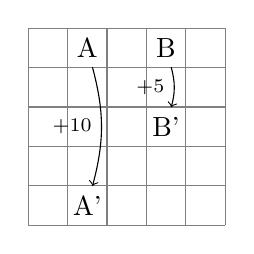
\begin{tikzpicture}
      \draw[step=0.5cm, color=gray] (0,0) grid (2.5,2.5);
      \node (A) at (0.75,2.25) {A};
      \node (A') at (0.75,0.25) {A'};
      \node (B) at (1.75,2.25) {B};
      \node (B') at (1.75,1.25) {B'};
      \draw [->][bend left=15] (A) edge node[left] {\scriptsize{+10}} (A');
      \draw [->][bend left=15] (B) edge node[left] {\scriptsize{+5}} (B');
    \end{tikzpicture}
    \caption{The simple gridworld Markov decision process.}
  \end{figure}
  The \emph{gridworld} MDP consist of 25 states $\cl{S} = [5]^2$ and 4 actions
  $\cl{A} = \{U, D, L, R\}$ for \emph{up}, \emph{down}, \emph{left} and 
  \emph{right}. The transition $P$ and reward $R$ kernels are deterministic:
  the agent moves 1 square up, down, left or right according to the chosen
  action and receives a reward of 0, except:
  \begin{itemize}
    \item Any move that would move the
      agent out of the grid results in no movement and a reward of -1.
    \item Any action in the state $A = (2,1)$ results in $A' = (2,5)$ as
      the next state and a reward of 10.
    \item Any action in the state $B = (4,1)$ results in $B' = (4,3)$ as
      the next state and a reward of 5.
  \end{itemize}
  Finally $\gamma = 0.9$ is the standard value of the discount factor
  in this example.
  Note that the discount factor is part of the definition of the environment,
  and thus the concept of optimality for the environment depends on the
  value of $\gamma$.

  Finite spaces are trivially standard Borel with the discrete topology,
  which also makes every map $(s, a) \mapsto \cl{X}$ into some
  topological space continuous. In particular $P$ is continuous and
  $r$ is (upper semi)continuous.
  The set of admissible actions $A(s)$ is equal to the
  full action space $\cl{A}$ for all $s \in \cl{S}$, which is trivially
  compact.
  The rewards are bounded by $R_{\max} = 10$
  and therefore $V_{\max} = 10/(1-0.9) = 100$.
  Thus we can apply \cref{cor:Viteration} and for $\wt{V}_0 = 0$ get that
  \[ \abs{\wt{V}_K - V^*} \leq \gamma^K \abs{V^*}
  \leq \gamma^K V_{\max} = 100 \cdot 0.9^{-K} \]
  
  By \cref{prop:propTpiV} for any stationary policy $\tau \in S\Pi$ we have
  that $T_\tau$ is also $\gamma$-contractive and we
  easily get the same bound on the policy evaluation
  \[ \abs{T_\tau^k V_0 - V_\tau} \leq \gamma^K V_{\max} \]
  To use \cref{alg:polEval} and \cref{alg:valueIteration} on the gridworld
  example we need to understand how the kernels $R, P$, value functions,
  policies and operators $T_\tau, T$ are represented in a computer.
  Since $\cl{S}$ and $\cl{A}$ are finite and small we can simply
  treat value functions $V$ as a vector $\wt{V} \in \R^{\cl{S}}$ and
  policies as a matrix of point probabilities
  $\wt{\tau} \in \R^{\cl{A} \times \cl{S}}$ so that
  $\wt{\tau}(a, s) = \tau(\{a\} \mid s)$.
  Since the rewards are deterministic
  the step $r \leftarrow \int x \difd R(x \mid \cdot)$ is irrelevant.
  $P$ is also deterministic so there exists a function
  $\wt{P} : \cl{S} \times \cl{A} \to \cl{S}$ such that
  $P(\{\wt{P}(s, a)\} \mid s, a) = 1$ for all $(s, a) \in \cl{S} \times \cl{A}$.
  Therefore the update step
  $\wt{V}_{k+1} \leftarrow T_\tau \wt{V}_k$ in \cref{alg:polEval}
  becomes
  \[ \text{For each} \; s \in \cl{S} :
    \wt{V}_{k+1}(s) \leftarrow
    \sum_{a \in \cl{A}}
  \left(r(s, a) + \gamma \wt{V}_k(\wt{P}(s,a)) \right) \wt{\tau}(a, s) \]
  Similarly in \cref{alg:valueIteration} the update step
  $\wt{V}_{k+1} \leftarrow T \wt{V}_k$ in \cref{alg:valueIteration}
  becomes
  \[ \text{For each} \; s \in \cl{S} :
    \wt{V}_{k+1}(s) \leftarrow
    \max_{a \in \cl{A}} \left(
  r(s, a) + \gamma \wt{V}_k(\wt{P}(s,a)) \right) \]

  Define the stationary policy $\tau_r(\cdot \mid \cdot) = \frac{1}{4}$ which
  chooses actions uniformly at random at every state.
  Below are shown some value functions of the gridworld environment
  (correct up to errors due to machine precision)
  found by applying 

  \begin{figure}[H]
    \centering
    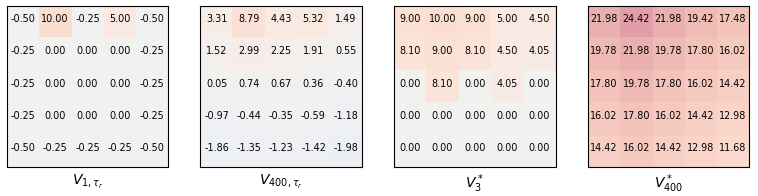
\includegraphics[scale=0.8]{figs/gridworld1.png}
    \caption{Value functions of the gridworld environment.
      Note that $V_{\max} \cdot \gamma^{400} = 100 \cdot (0.9)^{400}
      \approx 4.97 \cdot 10^{-17}$ so $V^*_{400}$ and $V_{\tau_r, 400}$
      are very close to the true infinite horizon value functions
    $V^*$ and $V_{\tau_r}$ (providing numerical errors are insignificant).}
    \label{fig:gw1}
  \end{figure}

  \begin{figure}[H]
    \centering
    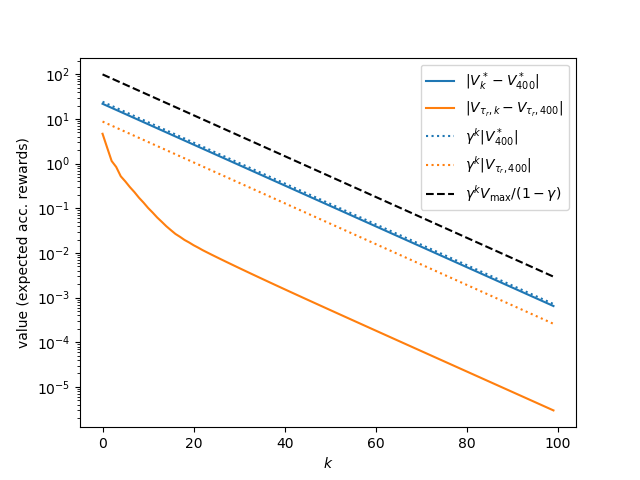
\includegraphics[scale=0.7]{figs/gridworld2.png}
    \caption{Convergence of gridworld value functions compared with
      the theoretical bounds. The black dashed line is the general theoretical
      bound for both $T$ and $T_{\tau}$ by Banachs fixed point theorem and
      the maximum value $V_{\max} = R_{\max} / (1-\gamma)$.
      The dotted blue and orange uses $\abs{V_k^*}$ and $\abs{V_{\tau, k}}$ 
      respectively, which might not be available.
    ($\gamma = 0.9$).}
    \label{fig:gw2}
  \end{figure}

  \label{ex:gridworld}
\end{example}

\subsection{Q-functions}

A \defemph{Q-function} is any function that assigns a real number
to every state-action pair, that is any function $Q : \cl{S} \times \cl{A}
\to \R$. Q-functions are also called \emph{action-value} functions,
to distinguish them from the \emph{value} functions we have discussed in the
previous sections.
The idea of Q-functions (and the letter Q) originates to
\mcite{W89}. Upon the definition he notes
\begin{displayquote}
  ``This is much simpler to calculate than [$V_\pi$]
  for to calculate [the greedy policy for $Q_\pi$] it is only necessary to look one
  step ahead [\ldots]''
\end{displayquote}
A clear advantage of working with Q-function
$Q:\Cal{S}\times\Cal{A} \to \Rext$ rather than a value function
$V:\Cal{S}\to \Rext$,
is that finding the optimal action $a^* \in A(s)$ at state $s$
requires only a maximization over the Q-function itself:
$a^* = \argmax_{a \in A(s)} Q(s,a)$.
This should be compared to finding an optimal action
according to a value function $V$:
$a^* = \argmax_{a \in A(s)} r(s,a) + \gamma \E_{P(\cdot \mid s,a)} V$.
Besides being less simple,
this requires taking an expectation with respect to 
both the reward and transition kernel.
Later we will study settings where we can only sample from $P$ and $R$
when attempting to find the optimal strategy.
In these situations the advantage of Q-functions is clear.
For now however the transition kernel will remain known and we
will in this section see how the results of state-value functions
translate to Q-functions.
Because of the similar role Q-functions play compared to value function,
many concepts such as $T$-operators and the finite, infinite horizon
policy evaluations and greedy policies, can be defined analogously.

\begin{asm}[Finite admissable actions]
  $A(s)$ is finite for every $s \in \cl{S}$. 
  \label{asm:finAdmAct}
\end{asm}
Throughout this section we will work under
\cref{sett:BS0} and \cref{asm:finAdmAct}.

\begin{rem}
  We make \cref{asm:finAdmAct} to ensure that the supremum
  $\sup_{a \in A(s)} Q(s, a)$ is attained for any
  $Q \in \cl{L}_\infty(\cl{S} \times \cl{A})$.
  One might be able discard \cref{asm:finAdmAct} and instead
  demand that all Q-functions be
  upper semicontinuous generalizing the discussion in this section.
  We have not pursued this generalization.
\end{rem}

\begin{defn}[Policy evaluation for Q-functions]
  Let $\pi \in R\Pi$.
  Define
  \[ Q_{k, \pi}(s, a) = r(s, a) + \gamma \E_{P(\cdot \mid s, a)} V_{k, \pi}
  ,\qquad Q_\pi(s, a) = r(s, a) + \gamma \E_{P(\cdot \mid s, a)} V_\pi \]
  \[ Q^*_k = \sup_{\pi \in R\Pi} Q_{k, \pi}
  , \qquad Q^* = \sup_{\pi \in R\Pi} Q_\pi \]
  Define $Q_0 = r$ then we make the convention that
  $Q^*_0 = Q_{0,\pi} = Q_0 = r$.
  \label{defn:polEvalQ}
\end{defn}

\begin{defn}[Operators for Q-functions]
  For any stationary policy $\tau \in S\Pi$ and
  integrable Q-function $Q:\Cal{S} \times \Cal{A} \to \R
  \in \cl{L}_\infty(\cl{S} \times \cl{A})$ we define
  \begin{align*}
    \text{Next-step operator: }
    P_\tau Q(s, a) &= \int Q(s', a') \difd \tau P(s', a' \mid s, a)
    \\ \text{Policy evaluation operator: }
    T_\tau Q(s, a) &= 
    r(s, a) + \gamma \int Q(s', a') \difd \tau P(s', a' \mid s, a)
    \\ \text{Bellman optimality operator: }
      T Q(s, a) &= r(s, a) + \gamma
    \int \max_{a' \in \Cal{A}} Q(s', a') \difd P(s' \mid s, a)
  \end{align*}
  where $T_a = T_{\delta_a}$.
  \label{defn:opQ}
\end{defn}
\begin{rem}
  The next-step operator $P_\tau$
  is defined for simplications in proofs, especially
  in the analysis of \mcite{F20} in the later sections.
  Using $P_\tau$ we can write $T_\tau$ alternatively as
  $T_\tau Q(s, a) = r(s, a) + \gamma P_\tau Q (s, a)$.
\end{rem}
\begin{defn}[Greedy policies for Q-functions]
  Let $\tau : \Cal{S} \leadsto \Cal{A}$ be a stationary policy. Define
  $G_Q(s) = \argmax_{a \in A(s)} Q(s, a)$.
  If there exist a measurable set $G_Q^\tau(s) \subseteq G_Q(s)$
  for every $s \in \Cal{S}$ such that
  \[ \tau \left( G_Q^\tau(s) \Mid s \right) = 1 \]
  then $\tau$ is said to be \defemph{greedy} with respect to $Q$ and is
  denoted $\tau_Q$.
  \label{defn:greedyQ}
\end{defn}

\begin{prop}[Relations between Q- and value functions]
  Let $\pi = (\tau_1, \tau_2, \dots) \in M\Pi$ be a Markov policy
  and $\tau \in S\Pi$ stationary. Then
  \leavevmode
  \begin{enumerate}
    \item Policy evaluations are related by
      $\E_{\tau(\cdot \mid s)} Q_{k, \pi} = V_{k+1, (\tau, \pi)}(s)$.
    \item $T_\tau$-operators are related by $T_\tau Q_{k, \pi}(s, a)
      = r + \gamma \E_{P(\cdot \mid s, a)} T_\tau V_{k, \pi}$.
    \item Greedy policies for policy evaluations are the same.
      That is
      \begin{enumerate}
	\item $\tau$ is greedy for
	  $Q_{k, \pi}$ if and only if $\tau$ is greedy for $V_{k, \pi}$.
	\item $\tau$ is greedy for $Q_\pi$ if and only if $\tau$ is greedy for
	  $V_\pi$.
      \end{enumerate}
    \item Optimal policies are related by
      $\max_{a \in A(s)} Q^*(s, a) = V^*(s)$ and
      \[ Q^*_k(s, a) = r(s, a) + \gamma \E_{P(\cdot \mid s, a)} V^*_k,
      \quad Q^*(s, a) = r(s, a) + \gamma \E_{P(\cdot \mid s, a)} V^* \]
    \end{enumerate}
  \label{prop:relQV}
\end{prop}

\begin{prop}[Properties of Q-functions]
  Let $\pi = (\tau_1, \tau_2, \dots) \in M\Pi$ be a Markov policy
  and $\tau \in S\Pi$ stationary. Then
  \leavevmode
  \begin{enumerate}
    \item $Q_{k, \pi} = T_{\tau_1} \dots T_{\tau_k} Q_0$ and
      $Q^*_k = T_{\tau_{k-1}^*} \dots T_{\tau_0^*} Q^*_0
      = T^k Q^*_0$.
    \item $Q_\pi = \lim_{k \to \infty} Q_{k, \pi}$ and
      $Q^* = \lim_{k\to\infty} Q_k^*$. 
    \item $T,\; T_\tau$ are $\gamma$-contractive on
      $\Cal{L}_\infty(\Cal{S}\times\Cal{A})$
      and $Q^*,\; Q_\tau$ are their unique fixed points.
    \item $Q^* = Q_{\tau^*}$ and
      $Q_{k, \pi},\; Q_\pi,\; Q^*_k,\; Q^*$ are all upper semicontinuous
      and bounded by $V_{\max}$.
  \end{enumerate}
  \label{prop:propQ}
\end{prop}

\begin{proof}[Proof of \cref{prop:relQV} and \cref{prop:propQ}]
%todo fix this proof
  Measurability of $Q_{k, \pi}$ and $Q_\pi$
  follow from measurability of $V_{k, \pi}$, $V_{\pi}$
  and \cref{prop:intKerMeas}.
  Upper semicontinuity of $Q_{k, \pi}$ and $Q_\pi$ follows
  from \cref{prop:intSemiC} because $V_{k, \pi}$ and $V_\pi$ are
  upper semicontinuous (see \cref{cor:Viteration}).

  For \cref{prop:relQV}.1 we have \begin{align*}
    \E_{\tau(\cdot \mid s)} Q_{k, \pi}
    &= \int r(s,a) + \gamma \E_{P(\cdot \mid s, a)} V_{k, \pi}
    \difd \tau(a \mid s)
    \\ &= \int r(s,a) + \gamma \sum_{i=1}^{k} \gamma^{i-1} r(s_i, a_i)
    \difd P \tau_k \dots P\tau_1 P\tau(a, s_1, a_1, \dots, s_k \mid s)
  \\ &= V_{k+1, (\tau, \pi)} \end{align*}
  
  For \cref{prop:relQV}.2 we sketch the idea by
  \begin{align*}
    T_\tau Q_{k, \pi} = r + \gamma \int r + \gamma V_{k, \pi}
    \difd P \difd \tau P
    = r + \gamma \int r + \gamma V_{k, \pi} \difd P \tau \difd P
    = r + \gamma \int T_\tau V_{k, \pi} \difd P
  \end{align*}
  
  For $Q_{k,\pi} = T_{\tau_1} \dots T_{\tau_k} Q_0$ use \cref{prop:relQV}.2
  iteratively starting with
  $\tau = \tau_1, \pi = (\tau_2, \tau_3, \dots)$.
  
  The $\tau(Q_{k, \pi}) = \tau(V_{k, \pi})$ part of \cref{prop:relQV}.3
  is by definition of the two concepts of
  greedy functions.

  That $Q_\pi = \lim_{k \to \infty} Q_{k, \pi}$
  follows from dominated convergence and
  \cref{prop:VpiMeas}.3.

  For \cref{prop:relQV}.4 $Q_k^* = \sup_{\pi \in R\Pi} (r + \gamma \E V_{k,\pi})
  \leq r + \gamma \E V_k^* = r + \gamma \E V_{\pi_k^*}
  \leq Q_k^*$. The same argument works for the second part.

  Let $s \in \Cal{S}$ then $\sup_{a \in A(s)} Q^*(s, a) = 
  \sup_{a \in A(s)} (r(s, a) + \gamma \E_{P(\cdot \mid s, a)} V^*)
  = T V^*(s) = V^*(s)$.
  
  By the definition of $Q_{\tau^*}$ we have
  $Q^* = r + \gamma \E V^* = r + \gamma \E V_{\pi^*} = Q_{\tau^*}$.

  $T_\tau Q_\tau = T_\tau (r + \gamma \E \lim_{k\to\infty} T_\tau^k V_0)
  = \lim_{k\to\infty} T_\tau (r + \gamma \E T_\tau^k V_0)
  = \lim_{k\to\infty} (r + \gamma \E T_\tau^{k+1} V_0)
  = r + \gamma \E \lim_{k\to\infty} T^{k+1}_\tau V_0
  = r + \gamma \E V_\tau = Q_\tau$.

    We $T_{\tau_Q} Q = T Q$ for any measurable $Q$ because
  \[ T_{\tau_Q}(s, a) = r(s, a) + \gamma \int \max_{a' \in A(s')} Q(s', a')
  \difd P(s' \mid s, a) = TQ(s, a) \]
  Therefore by \cref{prop:propQ}.1
  \[ T_{\tau_{k-1}^*} Q_{k-1, (\tau_{k-2}^*, \dots, \tau_0^*)}
  = T Q_{k-1}^* \]
  since by \cref{prop:relQV}.3 $\tau_{k-1}^*$ is greedy for $Q_{k-1}^*$.
  Now use induction to get $Q^*_{k-1} = T^k Q_0^*$.

  Because $V^* = V_{\tau^*}$ we have
  \[ TQ^* = T_{\tau^*} = r + \gamma \E T_{\tau^*} V_{\tau^*}
  = r + \gamma \E V^* = Q^* \]

  The contrativeness of $T$ and $T_\pi$ follows from the same argument as for
  value functions.
  Banach fixed point theorem now concludes \cref{prop:propQ}.3.

  Since now $Q^*$ and $Q_{\tau^*}$ are fixed points for $T$ they must be
  equal, concluding the last point, namely \cref{prop:propQ}.4.
\end{proof}

\subsubsection{Q-iteration}

Similar to the value iteration algorithm (\cref{alg:valueIteration}) we can
define the corresponding for Q-iteration.

\begin{figure}[H]
\begin{algorithm}[H] %\label{algocf:fq} % this labels line, could not fix
\caption{Simple theoretical Q-iteration}
\KwIn{MDP $(\Cal{S}, \Cal{A}, P, R, \gamma)$, number of iterations $K$}
Initialize the expected reward function:
$r \leftarrow \int x \difd R(x \mid \cdot)$.

Initialize the starting Q-estimator: $\wt{Q}_0 \leftarrow r$.

\For{$k = 0,1,2,\dots,K-1$}{
  Update the Q-estimator $ \wt{Q}_{k+1} = T \wt{Q}_k $
}
\KwOut{The $K$-optimal Q-function $Q^*_K = \wt{Q}_K$.}
\label{alg:theoSimpleQ}
\end{algorithm}
\end{figure}

By \cref{prop:propQ}.3 we thus have convergence of the \cref{alg:theoSimpleQ}:
\begin{cor}
  $\abs{Q^*_k - Q^*} \leq \gamma^k \norm{Q^*}_\infty
  \leq \gamma^k V_{\max}$.
  \label{prop:theoSimpleQConv}
\end{cor}

\subsection{Why are we not done?}

So far we have shown that value iteration under \cref{sett:BS0}
and Q-iteration under additionally \cref{asm:finAdmAct}, can solve
all such discounted MDPs with exponential convergence in $\gamma$.
This is a broad class of problems!
We name a few examples:
\begin{enumerate}
  \item Gridworld (\cref{ex:gridworld}).
  \item Board games like \emph{chess} and \emph{go}
    against a fixed (possibly randomized) opponent policy
    can be modelled accurately
    as such finite MDPs (putting $\gamma$ close to 1, so that winning late in 
    the game is still considered worth the effort).
  \item \emph{Pole balancing} in a 2D physical simulation environment
    (see e.g. the famous \emph{cartpole} example from \mcite{BSA83}).
    One may add random effects such and \emph{wind} to make such an example
\end{enumerate}
The problem is of course that the value functions and operators
which are used in \cref{alg:theoSimpleQ} are not computable in practice.
For example the state space of chess is very large
(roughly $\abs{\cl{S}_{\hrm{chess}}} \geq 10^{43}$).
This means that if we were to use \cref{alg:theoSimpleQ} naively
(with finite implementation as \cref{ex:gridworld})
then we would have to store a vector of
roughly $N \cdot 10^{43}$ real numbers for each Q-function we define,
where $N$ is the average number of admissable actions at each state
$\frak{A}(s), s \in \cl{S}$
which has been estimated to around $35$ for chess.
This requires roughly $1.4 \cdot 10^{45}$ bytes, if each number is stored as a
single precision floating point number (4 bytes).
For comparison the entire digital data capacity in the world is estimated
less than $10^{23}$ bytes as of 2020.
Needless to say this is beyond any practical relevance.

The rest of this thesis is therefore about the situations where we have
to use approximations and estimations for some or all of $P$, $R$ and
the Q-functions.

\section{Model-based Q-learning}
In this section we will look at what happens if we
instead use approximations of the Q-functions and $T$ operator.
This means that we are in a setting where we can somehow
calculate $r$ and $TQ$ for any $(s,a) \in \cl{S} \times \cl{A}$,
but it is hard or infeasible to represent them (or at least one of them)
directly.
The purpose of this is to show how results about the convergence of Q-learning
is rather easily obtained if one has direct access
to the transition and reward kernels $P$ and $R$.

It seems to this author,
that this setting is not very well-studied in the case of a
continuous state space.
This is perhaps because it is considered solved
by the results of theoretical Q-learning presented in the previous section.
However as we have argued, this only have practical relevance 
when it is feasible to represent $TQ$.
Therefore we find it relevant to consider this setting in more detail.

What \emph{is} very well-studied is a further generalized setting
where $T$ and $r$ are assumed to be unknown,
that is, one has only access to their distributions via sampling from them.
Solutions for that setting are called \emph{model-free}.
We will deal with that setting in the next section.

\subsection{Algorithmic and approximation errors}

In the following we present some rather simple bounding techniques
which is inspired by arguments found in e.g. \ncite{F20},
together with some standard results from approximation theory
on artificial neural networks and Bernstein polynomials.

Let us consider any norm $\norm{\cdot}$ on
the set of Q-functions $\cl{Q} = \{ f: \cl{S} \times \cl{A} \to \R \}$.
Let $\cl{F} \subseteq \cl{Q}$ be some subclass of Q-functions
Let $\wt{Q}_0 \in \cl{F}$ be bounded in $\norm{\cdot}$.
Suppose we can approximate $T\wt{Q}_0$ by some $\wt{Q}_1 \in \cl{F}$
to $\ve_1 > 0$ precision and then approximate $T\wt{Q}_1$ by $\wt{Q}_2 \in \cl{F}$
and so on. This way we get a sequence of Q-functions satisfying
\begin{equation}
\norm{T\wt{Q}_{k-1} - \wt{Q}_k} \leq \ve_k, \forall k \in \N
\label{eq:defnvei}
\end{equation}

First observe that
\begin{align*}
  \norm{T^k \wt{Q}_0 - \wt{Q}_k}
  &\leq \norm{T^k \wt{Q}_0 - T \wt{Q}_{k-1}} + \norm{T\wt{Q}_{k-1} - \wt{Q}_k}
  \\ &\leq \gamma \norm{T^{k-1} \wt{Q}_0 - \wt{Q}_{k-1}}
  + \norm{T\wt{Q}_{k-1} - \wt{Q}_k}
\end{align*}

Using this iteratively we get
\begin{equation}
  \norm{T^k \wt{Q}_0 - \wt{Q}_k} \leq \sum_{i=1}^k \gamma^{k-i} \ve_i
  \label{eq:mbitb}
\end{equation}
This is sometimes called the \defemph{approximation error}
and we denote it
\begin{equation}
  \ve_{\mathrm{approx}}(k) \defeq \sum_{i=1}^k \gamma^{k-i} \ve_i
  \label{eq:defapproxe}
\end{equation}

Thus we get
\begin{thm}
  Let $\norm{\cdot}$ be a norm on the space of functions
  $\cl{S} \times \cl{A} \to \Rext$.
  Let $\wt{Q}_k$ be obtained from a function class $\cl{F}$
  such that $\norm{\wt{Q}_{k} - T\wt{Q}_{k-1}} \leq \ve_k$
  for any $k \in \N$. Then
  \[ \norm{Q^* - \wt{Q}_k} \leq \gamma^k \norm{Q^* - \wt{Q}_0}
  + \ve_{\mathrm{approx}}(k) \]
  \label{thm:genApprox}
\end{thm}
\begin{proof}
  By the discussion above and
  \begin{align*}
    \norm{Q^* - \wt{Q}_k}
    &\leq \norm{Q^* - T^k \wt{Q}_0} + \norm{T^k \wt{Q}_0 - \wt{Q}_k}
    \\ &
    \stackrel{\ref{eq:mbitb}}{\leq}
    \gamma^k \norm{Q^* - \wt{Q}_0} + \ve_{\mathrm{approx}}(k)
  \end{align*}
\end{proof}
The first term in \cref{thm:genApprox} is sometimes called the
\defemph{algorithmic} error\footnote{For example in \ncite{F20}.}.
The algorithmic error converges exponentially, so one is usually happy with this
part not spending time trying to bound this tighter.
The approximation error depends on our step-wise approximations. For example
if $\ve_i(k) = \ve$ for some $\ve > 0$ we easily get the bound
\begin{equation}
  \ve_{\mathrm{approx}}(k) = \ve \frac{1-\gamma^k}{1-\gamma} \leq \frac{\ve}{1-\gamma}
  \label{eq:approxEpsBound}
\end{equation}
If $\ve_i \leq c\gamma^i$ we get $\ve_{\mathrm{approx}}(k) \leq ck \gamma^k \to 0$ as
$k \to \infty$.
Generally if one can show that $\ve_i \to 0$ we have
\begin{prop} $ \sum_{i-1}^k \gamma^{k-i} \ve_i \to 0 $
  whenever $\ve_k \to 0$ as $k \to \infty$.
\end{prop}
\begin{proof}
  Let $\ve > 0$. Find $N$ such that $\ve_n \leq \ve (1-\gamma)/2$ 
  for all $n>N$ and find $M>N$ such that
  $\gamma^M \leq
  \ve \gamma^N \left( \sum_{i=1}^N \gamma^{N-i} \ve_i \right)^{-1}$.
  Then for all $m>M$
  \begin{align*}
    \sum_{i=1}^m \gamma^{m-i} \ve_i
    &\leq \gamma^{m-N} \sum_{i=1}^N \gamma^{N-i} \ve_i
    + \sum_{i=N+1}^m \gamma^{m-i} \ve (1-\gamma)/2
    \leq \ve/2 + \ve/2 \leq \ve
  \end{align*}
\end{proof}
We will now explore two different ways of obtaining bounds on the approximation 
error.

\subsection{Using artifical neural networks}

\begin{sett}[Continuous MDP]
  An MDP $(\cl{S}, \cl{A}, P, R, \gamma)$ with
  $\cl{S} = [0,1]^w$, $\cl{A}$ finite and
  a continuous expected reward function $r$.
  \label{sett:annApprox}
\end{sett}

\begin{defn}\label{def_ANN}
  An \defemph{artificial neural network} (ANN) with $L \in \N_0$
  hidden layers, structure
  $(d_i)_{i=0}^{L+1} \subseteq \N$,
  activation functions $(\sigma_i)_{i=1}^L$,
  weights $(W_i)_{i=1}^{L+1} \in M^{d_i \times d_{i-1}}$ and
  biases $(v_i)_{i=1}^{L+1} \in \R^{d_i}$
  is the function $f:\R^{d_0} \to \R^{d_{L+1}}$ defined by
  \[ f = w_{L+1} \circ \sigma_L \circ w_L
  \circ \sigma_{L-1} \circ \dots \circ w_1 \]
  where $w_i$ is the affine function $x \mapsto W_i x + v_i$,
  and $\sigma_i : \R^{d_i} \to \R^{d_i}$ is coordinate-wise
  application of components $\sigma_{ij} : \R \to \R$.
  We denote the class of these networks (or functions)
  \[ \cl{DN} \left( (\sigma_i)_{i=1}^L,\; (d_i)_{i=0}^{L+1} \right) \]
  An ANN is called \emph{deep} if there are two or more hidden layers.
\end{defn}

We shall often consider networks with only one type of activation functions,
i.e. all activation functions are equal to one function $\sigma: \R \to \R$.
We then write $f \in \cl{DN}\left(\sigma, (d_i)_{i=0}^{L+1} \right)$ as a
shorthand.

\begin{figure}[h]
  \centering
  \tikzset{%
    every neuron/.style={
      circle,
      draw,
      minimum size=0.5cm
    },
    neuron missing/.style={
      draw=none, 
      scale=2,
      text height=0.2cm,
      execute at begin node=\color{black}$\vdots$
    },
  }
  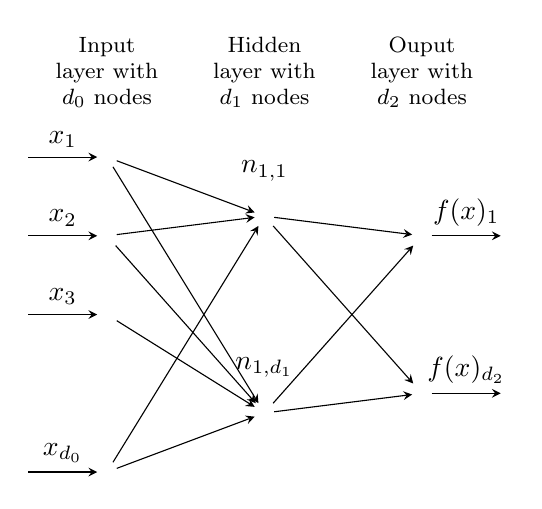
\begin{tikzpicture}[x=1cm, y=1cm, >=stealth]

    \foreach \m/\l [count=\y] in {1,2,3,missing,4}
    \node [every neuron/.try, neuron \m/.try] (input-\m) at (0,2.5-\y) {};

    \foreach \m [count=\y] in {1,missing,2}
    \node [every neuron/.try, neuron \m/.try ] (hidden-\m) at (2,2-\y*1.25) {};

    \foreach \m [count=\y] in {1,missing,2}
    \node [every neuron/.try, neuron \m/.try ] (output-\m) at (4,1.5-\y) {};

    \foreach \l [count=\i] in {1,2,3,d_0}
    \draw [<-] (input-\i) -- ++(-1,0)
    node [above, midway] {$x_{\l}$};

    \foreach \l [count=\i] in {1,d_1}
    \node [above=0.2cm] at (hidden-\i.north) { $n_{1, \l}$};

    \foreach \l [count=\i] in {1,d_2}
    \draw [->] (output-\i) -- ++(1,0)
    node [above, midway] {$f(x)_{\l}$};

    \foreach \i in {1,2,4} % 3 is looked at individually
    \foreach \j in {1,2}
    \draw [->] (input-\i) -- (hidden-\j);
      % 3
    \draw [->] (input-3) -- (hidden-2);

    \foreach \i in {1,...,2}
    \foreach \j in {1,...,2}
    \draw [->] (hidden-\i) -- (output-\j);

    \foreach \l [count=\x from 0] in {Input, Hidden, Ouput}
    \node [align=center, above, font=\footnotesize] at (\x*2,2)
    {\l \\ layer with \\ $d_{\x}$ nodes};
  \end{tikzpicture}
  \caption{An ANN with one hidden layer ($L=1$). Notice that there is no edge
    from $n_{0,3}$ to $n_{1,1}$ which means that
  $W_1(1,3) = 0$.}
\end{figure}

\begin{rem}
  Artificial neural networks are often illustrated as
  $L + 1$-partite graphs with $d_i$ nodes in the $i$th partition.
  A node $n_{i,j}$ in partition $i$ is then connected to a node
  $n_{i+1,k}$ if $W_{i+1}(k, j) \neq 0$.
  This is because they were
  inspired by the structure of \emph{neurons}
  in nerve tissue (e.g. the brain) of living organisms,
  with the graph nodes corresponding to neurons and edges to \emph{axons}.
  Indeed for every suitable collection of activation functions
  and every $L+1$-partite weighted graph $G$ satisfying
  \begin{equation}
    \text{\parbox{0.8\textwidth}{The $i$th partition is only
	connected to the neighboring $(i-1)$th and $(i+1)$th partition.
    }}
    \label{eq:graphANN}
  \end{equation}
  Then there exists a corresponding ANN corresponding to $G$.
  From the graph view-point it easy to see that one may join neural nets
  to form larger ones, by either function composition or side-by-side
  alignment.
  That this if
  $f \in \cl{DN}\left( (\sigma_i)_{i=1}^{L},\; (d_i)_{i=0}^{L + 1} \right)$
  and
  $g \in \cl{DN}\left( (\sigma'_i)_{i=1}^{L'},\; (d'_i)_{i=0}^{L' + 1} \right)$
  are two ANNs and $d_{L+1} = d_0'$ (i.e. that
  the dimensions match $\hrm{im}(f) \subseteq \hrm{dom}(g)$)
  then
  $g \circ f \in \cl{DN}
  \left( (\sigma_1, \dots, \sigma_L, \sigma'_1, \dots,
  \sigma'_{L'}), (d_1, \dots, d_L, d'_1, \dots, d'_{L'}) \right)$.
  By side-by-side alignment we mean the situation where $L = L'$
  and one creates the function
  $h : \R^{d_0 + d'_0} \to \R^{d_L + d'_L}$
  by defining $h(x_1, \dots, x_{d_0 + d'_0})
  = (f(x_1, \dots, x_{d_0}), g(x_1, \dots, x_{d'_0}))$.
  With this way of defining $h$ we have that
  $h$ is an ANN with structure $(d_0 + d'_0, \dots, d_{L+1} + d'_{L+1})$.
  Generally any way of stitching together graphs into $n$-partite graphs
  satisfying \cref{eq:graphANN}
  will gives ways of producing new ANNs. 
  \label{rem:annGraph}
\end{rem}

\begin{thm}[Universal Approximation Theorem for ANNs]
  Let $\sigma: \R \to \R$ be non-constant, bounded and continuous
  activation function.
  Let $\ve > 0$ and $f \in C([0,1]^w)$.
  Then there exists an $N \in \N$ and a network
  $F \in \cl{DN}(\sigma, (w, N, 1))$
  with one hidden layer,
  unbiased final layer (that is $v_2 = 0$)
  and activation function $\sigma$ such that
  \[ \norm{F - f}_\infty < \ve \]
  In other words $\bigcup_{N \in \N} \cl{DN}(\sigma, (w, N, 1))$ is
  dense in $C([0,1]^w)$.
  \label{thm:uniApprox}
\end{thm}
\begin{proof}[Discussion of proofs of \cref{thm:uniApprox}]
  The original proof in \mcite{C89} is very short and elegant,
  but non-constructive,
  using the Riesz Representation and Hahn-Banach theorems to
  obtain a contractiction to the statement that
  $\bigcup_{N \in \N} \cl{DN}(\sigma, (w,N,1))$
  is dense in $C([0,1]^w)$.
  Furthermore it considered only \emph{sigmoidal} activations
  functions, meaning that $\sigma$ should satisfy
  \[ \sigma(x) \to \begin{cases} 0 & x \to -\infty
  \\ 1 & x \to \infty \end{cases} \]
  
  This was extended in \mcite{CCR90} to the statement as presented above
  and their proof is constructive. 
\end{proof}

We will now show how ANNs can be used to approximate the optimal
value function to arbitrary precision,
and look at a particular class of ANNs called \emph{ReLU networks},
which are defined by their use of the \emph{ReLU activation function}
$\sigma_r(x) = \max(0, x)$.
We define the class of ReLU networks as the ANNs
with all ReLU activation functions, and write
$\cl{RN}\left( (d_i)_{i=0}^{L+1} \right)
\defeq \cl{DN}\left( \sigma_r, (d_i)_{i=0}^{L+1} \right)$.

\begin{prop}
  Under \cref{sett:annApprox} let $\varepsilon > 0$.
  Assume that either
  \begin{enumerate}
    \item $P$ is deterministic with $P(\cdot \mid s, a) = \delta_{p(s, a)}$.
      For some continuous $p: \cl{S} \times \cl{A} \to \cl{S}$.
  \end{enumerate}

  or
  \begin{enumerate}[resume]
    \item $P(\cdot \mid s, a)$ is absolutely continuous
      with respect to the same measure $\nu$ on $\cl{S}$ for all
      $(s, a) \in \cl{S} \times \cl{A}$ with density
      $p(\cdot \mid s, a)$ which is continuous in $s$.
  \end{enumerate}
  Then for every $k \in \N$ there exists a $N\in \N$ and a sequence of
  Q-networks $(\wt{Q}_i)_{i=1}^k \subseteq \cl{RN}(w \abs{\cl{A}}, N, 1)$
  such that
  \[ \ve_{\mathrm{approx}}(i) = \norm{T\wt{Q}_{i-1} - \wt{Q}_i}_\infty < \ve \]
  for all $i \in [k]$.
  In particular
  \[ \abs{Q^* - \wt{Q}_k} < \varepsilon/(1 - \gamma) \]
\end{prop}
\begin{proof}[Proof]
  The key points are that
  \begin{enumerate}[label=\alph*.]
    \item Any ANN with continuous activation functions is continuous.
    \item Under assumptions 1. or 2. the Bellman operator $T$ preserves
      continuity.
    \item It is possible to join a finite number of ReLU networks
      $f_{a_1}, \dots, f_{a_\frak{a}} : \cl{S} \to \R$
      into a bigger ReLU network $f : \cl{S} \times \cl{A} \to \R$
      such that $f(s, a) = f_a(s)$.
  \end{enumerate}

  Using these facts we can use the universal approximation theorem
  (\cref{thm:uniApprox}) to get a series of networks
  \[ f_{a, k} : \cl{S} \to \R \]
  for each $a \in \cl{A}$ and $k \in \N$ satisfying
  \begin{equation}
    \abs{f_{a, k} - T \wt{Q}_{k-1}(\cdot, a)} < \ve
    \label{eq:ann_approx_1}
  \end{equation}
  Here $\wt{Q}_0 = r$ and $\wt{Q}_k$ is obtained recursively by
  joining for each $a$ the components $f_{a, k}$ into a single network
  $\wt{Q}_k : \cl{S} \times \cl{A} \to \R$ such that
  $\wt{Q}_k(s, a) = f_{a, k}(s)$.
  By \cref{eq:ann_approx_1} on each of its components
  approximates $T \wt{Q}_{k-1}$ to $\ve$ precision.
  $\wt{Q}_0$ is continuous by \cref{sett:annApprox} and by
  a. and b. $T \wt{Q}_k$ is as well.
  
  We will now establish points a., b. and c.
  \begin{enumerate}[label = \alph*.]
  \item follows by the fact that that composition of continuous functions
    are continuous.
  \item Let $Q: \cl{S} \times \cl{A} \in \cl{L}_\infty(\cl{S} \times \cl{A})$
    be continuous and let
    $x_1, x_2, \dots \in \cl{S} \times \cl{A}$ with
    $x_\ell \to x \in \cl{S} \times \cl{A}$.
    We will show that
    under 1. or 2. we have $TQ(x_\ell) \to TQ(x)$.
    \begin{enumerate}[label = \arabic*.]
      \item In this case $TQ(x) = r(x) + \gamma
	\max_{a' \in \cl{A}} Q(p(x), a')$ can be seen as the composition
	of the continuous functions $p$, $Q$, $\max$, $+$ and $r$.
      \item We have by dominated convergence and the assumption that
	$r$ is continuous (see \cref{sett:annApprox}) that
	\begin{align*}
	  TQ(x_\ell) &= r(x_\ell) + \gamma \int \max_{a'\in \cl{A}}
	  Q(s', a') p(s' \mid x_\ell) \difd v(s')
	  \\ &\to r(x) + \gamma \int \max_{a'\in \cl{A}}
	  Q(s', a') p(s' \mid x) \difd v(s')
	  \\ &= TQ(x)
	\end{align*}
    \end{enumerate}
  \item Let $k \in \N$.
    To join the components $f_{a, k}$ into a single network
    we embed $\cl{A}$ into $[0,1]^\frak{a}$ (where $\abs{\cl{A}} = \frak{a}$)
    by enumerating the actions $\cl{A} = \{ a_1, a_2, \dots, a_\frak{a} \}$
    and putting $a_i = (0,\dots,0,1,0,\dots,0)$ where the 1 is on the $i$th
    spot (this is called the \emph{one-hot embedding}).
    Let $L_a, (d_{a, i})_{i=0}^{L_a + 1}$ denote the number of hidden layers 
    and structure of $f_{a, k}$.
    We can now define $\wt{Q}_k : [0,1]^{w + \frak{a}} \to \R$
    as the ReLU network with 
    $L = 2 + \max_{a \in \cl{A}} L_a$ hidden layers and structure
    $d_0 = w + \frak{a}$, $d_1 = w \cdot \frak{a}$ and
    $d_i = \sum_{a \in \cl{A}} d'_{a, i-1}$ for $i = 2, \dots L-1$ putting
    $d'_{a, i} = d_{a, i}$ for $1 \leq i \leq L_a - 1$
    and $d'_{a, i} = d_{a, L_a}$ for $L_a \leq i \leq L - 1$
    then $d_L = \frak{a}$
    and finally $d_{L + 1} = 1$.
    The first layer consist of the affine map
    $w_1 : \R^{w + \frak{a}} \to \R^{w \cdot \frak{a}}$ defined by
    \[ w_1(s, 0, \dots, 1, \dots, 0)
    = (s, \dots, s + 1, \dots, s) - 1 \]
    where $s = (s_1, \dots, s_w) \in \R^w$ and where
    we use the notation $1 = (1, \dots, 1) \in \R^k$ for any $k \in \N$.
    Applying the ReLU activation $\sigma_r = \max(0, \cdot)$
    coordinate-wise we get
    \[ \sigma_r(w_1(s, 0, \dots, 1, \dots, 0)) =
    (0, \dots, s, \dots, 0) \]
    since all $s_i \in [0,1]$, so $\max(0, s_i - 1) = 0$ and
    $\max(0, s_i) = s_i$.
    We now use the component networks middle part of the network of $\wt{Q}_k$.
    For $2 \leq i \leq L$ put
    $w_i = (w_{1, i-1}, \dots, w_{\frak{a}, i-1}) : \R^{d_{i-1}} \to \R^{d_i}$ 
    where we define
    \[ w_{j, i} = \begin{cases}
	\text{the $i$th affine map of } f_{a_j, k} & 1 \leq i \leq L_{a_j}
	\\ \text{the identity map: } 
	\id : \R^{d_{a_j, i-1}} \to \R^{d_{a_j, i}} & L_{a_j} < i < L
	\\ \text{the $i$th affine map of } f_{a_j, L_{a_j} + 1} & i = L
	\\ \text{summation: } (x_1, \dots, x_\frak{a}) \mapsto
	\sum_{\ell = 1}^\frak{a} x_\ell & i = L + 1
    \end{cases} \]
    With this construction we have that
    $\wt{Q}_k(s, a) = f_{a, k}(s)$
    for all $a \in \cl{A}$.
    And that $\wt{Q}_k(s, a) \in \cl{RN}(w + \frak{a}, w\cdot \frak{a}
    , d_2, \dots, d_{L-1}, d_\frak{a}, 1)$.
\end{enumerate}
\end{proof}

This gives us the first method of how to approximate
$Q^*$ arbitrarily closely on continuous state spaces, in the case
where it is infeasible to represent $TQ$ directly.
However it is still not clear if this method is feasible
computationally.
To investigate this and indeed for any chance to implement the method
in practice one would need to go through the
construction in \ncite{CCR90}. We will not go further into this,
and instead focus on another approximation method using
\emph{Bernstein polynomials}.

\subsection{Using Bernstein polynomials}

In this case we need a stronger form of continuity, namely
Lipschitz continuity (see \cref{defn:Lipschitz}), to establish the bounds.

\begin{sett}[Bernstein approximable MDP]
  An MDP $(\cl{S}, \cl{A}, P, R, \gamma)$ with
  $\cl{S} = [0,1]^w$ and $\cl{A}$ finite.
  Assume that there exists a probability measure $\mu \in \cl{S}$, such that
  $P(\cdot \mid s, a)$ has density
  $p(\cdot \mid s, a) : \cl{S} \to \R$ with respect to
  $\mu$ for all $(s, a) \in \cl{S}\times\cl{A}$. 
  Furthermore assume that $r(\cdot, a), \; p(s \mid \cdot, a)$ are
  $\norm{\cdot}$-Lipschitz
  with constants $L_r,\; L_p$ respectively for all
  $(s, a) \in \cl{S} \times \cl{A}$
  for some norm $\norm{\cdot}$.
  \label{sett:polyApprox}
\end{sett}

\begin{defn}[Bernstein polynomial]
  The (multivariate) Bernstein polynomial $B_{f, n}$ of degree
  $n=(n_1, \dots, n_w) \in \N^w$ approximating the function $f:[0,1]^w \to \R$
  is defined by
  \begin{equation*}
    B_{f, n}(x_1, \dots, x_w) =
    \sum_{j = 1}^w \sum_{k_j = 0}^{n_j}
    f\left( \frac{k_1}{n_1}, \dots, \frac{k_w}{n_w} \right)
    \prod_{\ell = 1}^w \left(
    \binom{n_\ell}{k_\ell} x_\ell^{k_\ell}(1-x_\ell)^{n_\ell - k_\ell} \right)
  \end{equation*}
  \label{defn:Bfn}
\end{defn}
Notice that this a polynomial of (multivariate) degree
$\norm{n}_1 = n_1 + \dots + n_w$.

\begin{thm}[Approximation with Bernstein polynomials]
  Let $f : [0,1]^w \to \R$ be Lipschitz
  w.r.t. the standard euclidean 2-norm induced metrics on $[0,1]^w$ and $\R$
  with constant $L$. 
  Let $n = (n_1, \dots, n_w) \in \N^w$.
  The Bernstein polynomial
  $B_{f,n} : [0,1]^w \to \R$ satisfies
  \begin{enumerate}
    \item $\norm{f - B_{f,n}}_\infty
      \leq \frac{L}{2} \sqrt{\sum_{j=1}^w \frac{1}{n_j}}$
    \item $\norm{B_{f,n}}_\infty \leq \norm{f}_\infty$
  \end{enumerate}
  \label{thm:bernsteinApprox}
\end{thm}
\begin{proof}
  We refer to \mcite{H02} thm. B..7.
\end{proof}

\begin{lem}
  Under \cref{sett:polyApprox} 
  $TQ(\cdot, a)$ is Lipschitz in $\norm{\cdot}_2$ with constant
  $ L_T = L_r + \gamma V_{\max} L_p $
  for all $a \in \cl{A}$ and measurable
  $Q : \cl{S} \times \cl{A} \to [-V_{\max},V_{\max}]$.
  \label{lem:bernsteinLem}
\end{lem}
\begin{proof}
  Because of the Lipschitz property of $r$ and $p$ we have
  for any measurable $Q : \cl{S} \times \cl{A} \to [-V_{\max},V_{\max}]$
  and $s \neq s' \in \cl{S}$ that
  \begin{align*}
    \abs{TQ(s, a) - TQ(s', a)}
    &\leq \abs{r(s, a) - r(s', a)} 
    \\ &+ \gamma \int
    \abs{\max_{a'\in\cl{A}}Q(s'', a') p(s'' \mid s, a)
    - \max_{a'' \in \cl{A}} Q(s', a'') p(s'' \mid s', a) }
    \difd \mu(s'')
    \\ &\leq L_r \norm{s - s'} + \gamma \int
    \abs{\max_{a'\in\cl{A}}Q(s', a')}
    \abs{p(s'' \mid s, a) - p(s'' \mid s', a)}
    \difd \mu(s'')
    \\ &\leq L_r \norm{s - s'} + \gamma \int
    V_{\max}
    L_p \norm{s - s'}
    \difd \mu(s'')
    \\ & = (L_r + \gamma V_{\max} L_p) \norm{s - s'}
  \end{align*}
\end{proof}

Now we can bound

\begin{prop}
  Given an MDP satisfying \cref{sett:polyApprox} and using $\norm{\cdot}_\infty$
  we can bound
  \[ \ve_{\mathrm{approx}} \leq \frac{L_r + \gamma V_{\max} L_p}{2(1-\gamma)}
  \sqrt{\sum_{j=1}^w \frac{1}{n_j}} \]
  \label{prop:veapproxlibbound}
\end{prop}
\begin{proof}
  Following the procedure from leading to \cref{eq:mbitb},
  starting with $\wt{Q}_0 = 0$
  and using the $n = (n_1, \dots, n_w)$ degree Bernstein polynomium
  $\wt{Q}_{k} = B_{T\wt{Q}_{k-1}, n}$ as approximation for $T\wt{Q}_{k-1}$
  we know by induction and
  the results \cref{lem:bernsteinLem}
  and \cref{thm:bernsteinApprox}.2 that $T\wt{Q}_k$ is
  $L_T$-Lipschitz for any $k \in \N$.
  Now by choosing the euclidean norm $\norm{\cdot} = \norm{\cdot}_2$
  we have by \cref{thm:bernsteinApprox}.1 that
  \begin{equation}
    \ve_i = \norm{\wt{Q}_k - T\wt{Q}_{k-1}}_\infty
    \leq \frac{L_T}{2} \sqrt{\sum_{j=1}^w \frac{1}{n_j}} = \ve
    \label{eq:veapproxlib1}
  \end{equation}
  where $\ve$ is the one-step error defined in \cref{eq:defnvei}.
  Now by \cref{eq:approxEpsBound}
  we have that
  \begin{equation}
    \ve_{\hrm{approx}} \leq \frac{\ve}{1-\gamma}
    \label{eq:veapproxlib2}
  \end{equation}
  Combining \cref{eq:veapproxlib1} and \cref{eq:veapproxlib2} and noting
  that $L_T = L_r + \gamma V_{\max} L_p$ finishes the proof.
\end{proof}

To make more clear what are the implications of \cref{prop:veapproxlibbound}
we give a corollary where we put $n_j = m$ for all $j \in [w]$:

\begin{cor}
  Under \cref{sett:polyApprox} and using Bernstein polynomials of degree
  $n = (m, \dots, m) \in \N^w$ for $m \in \N$ we have the following bound
  \[ \norm{Q^* - \wt{Q}_k}_\infty \leq \gamma^{-k} V_{\max}
    + \frac{L_r + \gamma V_{\max} L_p}{2(1-\gamma)} \sqrt{w}
  \frac{1}{\sqrt{m}} \]
  In particular $\norm{Q^* - \wt{Q}_k}_\infty
  = \cl{O}(\gamma^{-k} + \frac{1}{\sqrt{m}})$
  when using $k$ iterations.
  \label{cor:libbound}
\end{cor}
\begin{proof}
  Use \cref{prop:veapproxlibbound}.
\end{proof}

This gives a very concrete way of constructing an arbitrarily good
approximation to $Q^*$ using polynomials.
A major drawback is the restriction on the transition dynamics $P$.
For example we cannot use \cref{cor:libbound} on deterministic
decision processes, since if $P$ is deterministic then there
are no measure $\mu \in \cl{P}(\cl{S})$ which allows for a
density $p(\cdot \mid s, a)$ (i.e. $p \cdot \mu = P(\cdot \mid s, a)$),
unless $P(\cdot \mid s, a) = \delta_{s'}$ for all $(s, a) \in \cl{S} \times
\cl{A}$, which would lead to a quite boring environment.
Generally the processes with fast convergence bounds 
according to \cref{cor:libbound} must be very stochastic.
%todo example.

This concludes our investigation of model-based Q-learning and we will
now look at the much more well-studied field of model-free Q-learning.

